\documentclass[10pt,twocolumn]{article}
\usepackage{geometry}
\geometry{verbose,headsep=3cm,tmargin=2.5cm,bmargin=2.5cm,lmargin=2.0cm,rmargin=2.0cm}
\usepackage{graphicx}
\usepackage{xcolor}
\usepackage[font=small]{caption}
\usepackage{amsmath,amssymb,latexsym}
\usepackage{marvosym}
\usepackage{url}
\usepackage{lipsum}
\usepackage{bm}
\usepackage{float}
\usepackage[english]{babel}
\usepackage{hyperref}
\usepackage{subcaption}
\usepackage{subfloat}
\usepackage{epsf}
\usepackage{float}
\usepackage{mathpazo}
\usepackage{pifont}
\usepackage{wrapfig}
\usepackage{multicol}
\usepackage{enumitem}
\usepackage{xcolor}
\usepackage{framed}
\usepackage[utf8]{inputenc}
\graphicspath{{DWGs/}}
\usepackage{framed}
\usepackage{textcomp}
\usepackage{braket}
\newcommand{\highlight}[1]{%
  \colorbox{orange!50}{$\displaystyle#1$}}
% Default fixed font does not support bold face
\DeclareFixedFont{\ttb}{T1}{txtt}{bx}{n}{10} % for bold
\DeclareFixedFont{\ttm}{T1}{txtt}{m}{n}{10}  % for normal

% Custom colors
\usepackage{color}
\definecolor{deepblue}{rgb}{0,0,0.5}
\definecolor{deepred}{rgb}{0.6,0,0}
\definecolor{deepgreen}{rgb}{0,0.5,0}

\usepackage{listings}

% Python style for highlighting
\newcommand\pythonstyle{\lstset{
language=Python,
basicstyle=\ttm,
otherkeywords={self},             % Add keywords here
keywordstyle=\ttb\color{deepblue},
emph={MyClass,__init__},          % Custom highlighting
emphstyle=\ttb\color{deepred},    % Custom highlighting style
stringstyle=\color{deepgreen},
frame=tb,                         % Any extra options here
showstringspaces=false            % 
}}


% Python environment
\lstnewenvironment{python}[1][]
{
\pythonstyle
\lstset{#1}
}
{}

% Python for external files
\newcommand\pythonexternal[2][]{{
\pythonstyle
\lstinputlisting[#1]{#2}}}

% Python for inline
\newcommand\pythoninline[1]{{\pythonstyle\lstinline!#1!}}
% Document font:
\usepackage{charter}

\begin{document}

%%% HEADER --------------------------------------------------------------
% ------------------------------------------------------------------------

\twocolumn[{
\begin{@twocolumnfalse}

  \begin{center}
%\textcolor{lgray}
    \vskip-5em

    \hfill
    \fontsize{10}{10}\selectfont {\textit{Bruxelles, October 2019 - Salt Lake City, March 2020}}
    \vskip2ex
	\vspace{5ex}
    \fontsize{20}{10}\selectfont {The linear algebra of Principal Component Analysis}
      \vspace{1ex}
      
      \fontsize{16}{10}\selectfont {(with Python examples)}
  \noindent%
    
\vskip1ex

{\rule{\textwidth}{0.5pt}}

  \end{center}
  
    \fontsize{7}{10}\selectfont {This work is licensed under the Creative Commons Attribution-NonCommercial-ShareAlike 4.0 International (CC BY-NC-SA 4.0) license.}

\vspace{6mm}

\end{@twocolumnfalse}
}]

%%% HEADER END -----------------------------------------------------------
% ------------------------------------------------------------------------

\vspace{10mm}

\setlength{\parindent}{0cm}

\fontsize{14}{10}\selectfont {Kamila Zdybał}

\vspace{2mm}

\fontsize{8}{10}\selectfont {\textit{Université libre de Bruxelles, kamila.zdybal@ulb.ac.be}}

\fontsize{8}{10}\selectfont {\textit{camillejr.github.io/science-docs, kamila.zdybal@gmail.com}}

\section*{Preface}

\textbf{Principal Component Analysis} (PCA) is a multivariate dimensionality reduction technique in which a high-dimensional data set is projected on directions of decreasing importance, ordered by the amount of variance explained. The technique exploits the fact that the original basis to represent the data set might not be an \textit{optimal} one and there might be a redundancy of dimensions. Once a new, orthogonal basis is found, the data can be transformed to that new basis and that can give certain advantages. The projected data has lower rank and is thus easier to analyze. This in turn can be helpful in a variety of problems such as extracting information, data compression or analysis of structures hidden in the data \cite{Abdi_Williams}.

\,\,

These notes are in a way a tutorial on PCA with a deeper focus on linear algebra and statistics aspects governing this method. The aim is to present a deeper understanding of several linear algebra concepts than some quick online tutorials would give. My goal was also to gather all important knowledge on PCA in one place. 

\,\,

The prerequisite for these notes is mainly familiarity with undergraduate level linear algebra. You should be comfortable with the concept of matrices and operations on matrices. You will profit more from these notes if you have an intuitive understanding of eigendecomposition. If you need a refresher, the excellent series on linear algebra by 3Blue1Brown will be, in my opinion, everything you need to go through these notes \cite{3Blue1Brown}. In addition, some easy concepts from statistics such as variance and covariance will be used.

\,\,

This document is still in preparation. Please feel free to contact me with any suggestions, corrections or comments.

\section*{Keywords}

\textit{principal component analysis, data reduction, dimensionality reduction, linear algebra, MATLAB\textregistered, Python}

\tableofcontents

\section*{Nomenclature}

\begin{tabular}{ll}
    $\bm{A}$ & is a matrix \\
     $\bm{A}^T$ & is a matrix transpose \\
     $\bm{a}$ & is a vector \\
     $a$ & is a scalar \\
    $\bm{a}_j$ & is the $j^{th}$ column of a matrix $\bm{A}$, \\
    & it is equivalent to  $\bm{A}(:,j)$ \\
    $\bm{a}_i$ & is the $i^{th}$ row of a matrix $\bm{A}$, \\
    & it is equivalent to  $\bm{A}(i,:)$ \\
    $a_{i,j}$ & is an element from $i^{th}$ row and $j^{th}$ column of a matrix $\bm{A}$, \\ 
    & it is equivalent to  $\bm{A}(i,j)$ \\
\end{tabular}

%\section{Motivation for data reduction}
%
%To motivate why studying techniques such as PCA and learning to apply them on real data sets is important, there are several questions which stimulated the development of data reduction and data decomposition techniques:
%
%\begin{enumerate}
%\item Can we send less data but preserve maximum information contained by the data (data compression)?
%
%\item Can we predict what the outcome of another observation will be?
%
%\item Can we build a model in a purely data-driven way - based on data that we have collected (e.g. from experiments or numerics)?
%
%\item Can we make sense of a large, multi-dimensional data set (which cannot be plotted graphically)?
%
%\item Can we extract low-dimensional features that underlay the data?
%\end{enumerate}
%
%All of these questions are not necessarily answerd by PCA. Different applications might work well with different data reduction techniques.

\section{Data sets for PCA}

For the rest of this document, we assume that the data set for performing PCA is a matrix $\bm{X}$. Each column of $\bm{X}$ represents all observations of one variable (feature). Each row of $\bm{X}$ corresponds to a single observation (sample) of all variables. Let $i \in \braket{1, n}$ index the observations and $j \in \braket{1, Q}$ index the variables. The data matrix $\bm{X}$ is hence size $(n \times Q)$.\footnote{This is also the data format that is needed for the MATLAB\textregistered \, function \texttt{pca} \cite{Matlab-pca} and for the Python function \texttt{sklearn.decomposition.PCA} \cite{Python-pca}.} This structure can be seen in Fig.\ref{fig:data-matrix}.

%One of the strengths of PCA is that it can be performed on a non-time-resolved data set, namely the matrix $\bm{X}$ can be collected at a single time snapshot and be only spatially-resolved.

\begin{figure}[H]
\centering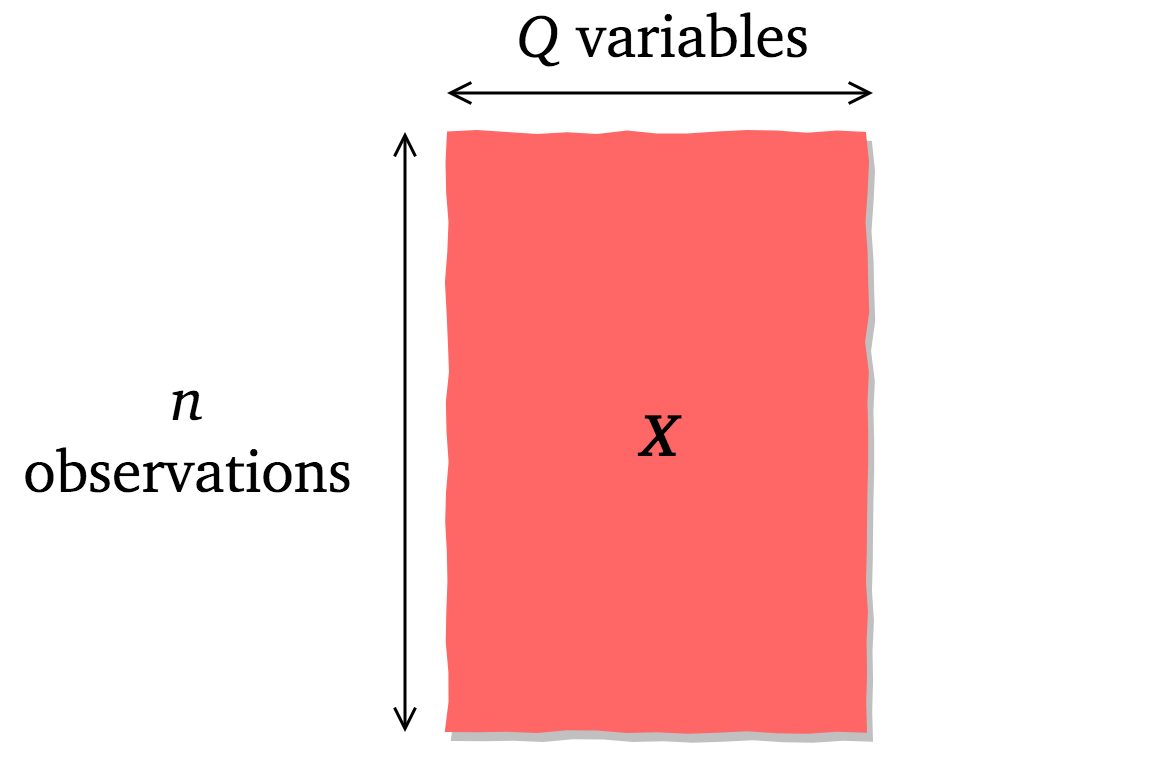
\includegraphics[width=5cm]{data-set-PCA.png}
\caption{Data matrix for PCA.}
\label{fig:data-matrix}
\end{figure}

\section{Data pre-processing}

In data science we are typically given a raw data set which is not centered and not scaled. However, standardizing the data set might be a good idea before applying a data science technique.

In particular, \textit{centering} allows to look at data as variations from some center. Graphically, centering shifts the center of the \textit{cloud} of data points (which in general is multi-dimensional) to a new, selected center. One of the popular choices is to center each variable by subtracting the mean of this variable's observations - the center will be shifted to the origin\footnote{see Fig.\ref{fig:python-raw-data}-\ref{fig:python-raw-data-centered}.}.
Other centering that could be encountered\footnote{for instance in the \textit{Min-Max} standardizing.} is subtracting the minimum of the variable's observations.

Centering thus substitutes the original data set with:

\begin{equation}
\bm{X_c} = \bm{X} - \bm{C}
\end{equation}

Here, a matrix of centers $\bm{C}$ is created, for instance by computing the mean of each column of $\bm{X}$. In that case, a single column of $\bm{C}$ is populated with the same value representing the mean of the corresponding column in $\bm{X}$. $\bm{C}$ is thus also size $(n \times Q)$. A specific center $\bm{c}_j$ is then subtracted from a corresponding column $\bm{x}_j$.

\textit{Scaling}, on the other hand, allows us to cancel the effect of various ranges that the variables in the data set might have, and treat all variables with equal (or at least similar) importance. A centered and scaled data set can then be written as follows:

\begin{equation}
\bm{X_{cs}} = \bm{X_c}\bm{D}^{-1}
\end{equation}

In the above equation, matrix $\bm{D}$ is a diagonal matrix whose entries are the corresponding scalings. Hence, every column of $\bm{X_c}$ gets divided by a corresponding scale from the diagonal of matrix $\bm{D}$.

One of the popular scaling methods used in literature is the \textit{auto scaling}\footnote{also known as \textit{standard scaling} or \textit{z-score} (although \textit{z-score} refers to a combination of centering by mean and scaling with a standard deviation).} in which each column is divided by the standard deviation of that column. After auto scaling all columns have a standard deviation equal to 1.

To further motivate data scaling with an illustrative example, you might think of a set of variables from a single experiment, representing temperature in the units of $[K]$ and range from 300-1500 $K$ and associated pressures in the units of $[atm]$ which range from 1-1.1 $atm$. If we did not scale the data, the largest \textit{spread} or the \textit{variance} would be found in temperature, since on purely numerical grounds, the range 300-1500 is more significant than the range 1-1.1.

For simplicity, for the rest of this document we assume that $\bm{X}$ represents already pre-processed data (in place of $\bm{X_{cs}}$).

\section{Covariance matrix}

The covariance between two random vectors $\bm{x}$ and $\bm{y}$ is defined as:

\begin{equation}\label{eq:covariance-definition}
\text{cov}(\bm{x},\bm{y}) = \frac{1}{n} \sum_{i=1}^{n} (x_i - \bar{\bm{x}}) (y_i - \bar{\bm{y}})
\end{equation}

where $n$ is the number of samples (weights of a vector). If we look at any data matrix as a composition of vectors formed by its columns, we may compute the covariances of these vectors and store the result in another matrix, called a \textit{covariance matrix}. This matrix is symmetric due to symmetry: $\text{cov}(\bm{x},\bm{y}) = \text{cov}(\bm{y},\bm{x})$. The off-diagonal elements have the meaning of covariance of two random vectors and the elements on the diagonal represent variance of each corresponding column, since $\text{cov}(\bm{x},\bm{x}) = \text{var}(\bm{x})$ where:

\begin{equation}\label{eq:variance-definition}
\text{var}(\bm{x}) = \frac{1}{n} \sum_{i=1}^{n} (x_i - \bar{\bm{x}})^2
\end{equation}

\subsection{Construction}

The starting point for performing PCA is to compute a covariance matrix from the data set. The covariance matrix is given by:

\begin{equation}\label{eq:cov-matrix}
\bm{S} = \frac{1}{n-1} \bm{X}^T \bm{X}
\end{equation}

and is therefore size $(Q \times Q)$. Notice the similarity with the eq.(\ref{eq:covariance-definition}).

We will start by exploring the meaning of $\bm{X}^T \bm{X}$. Let's look at the graphical representation of this matrix multiplication in Fig.\ref{fig:covariance-matrix}.

Any given column, say $p$ or $k$, of the data matrix $\bm{X}$ represents all measurements of a single $p^{th}$ (or $k^{th}$) variable and can be viewed as an $n$-dimensional vector. The same can be said about any row of a matrix $\bm{X}^T$.

\begin{figure}[H]
\centering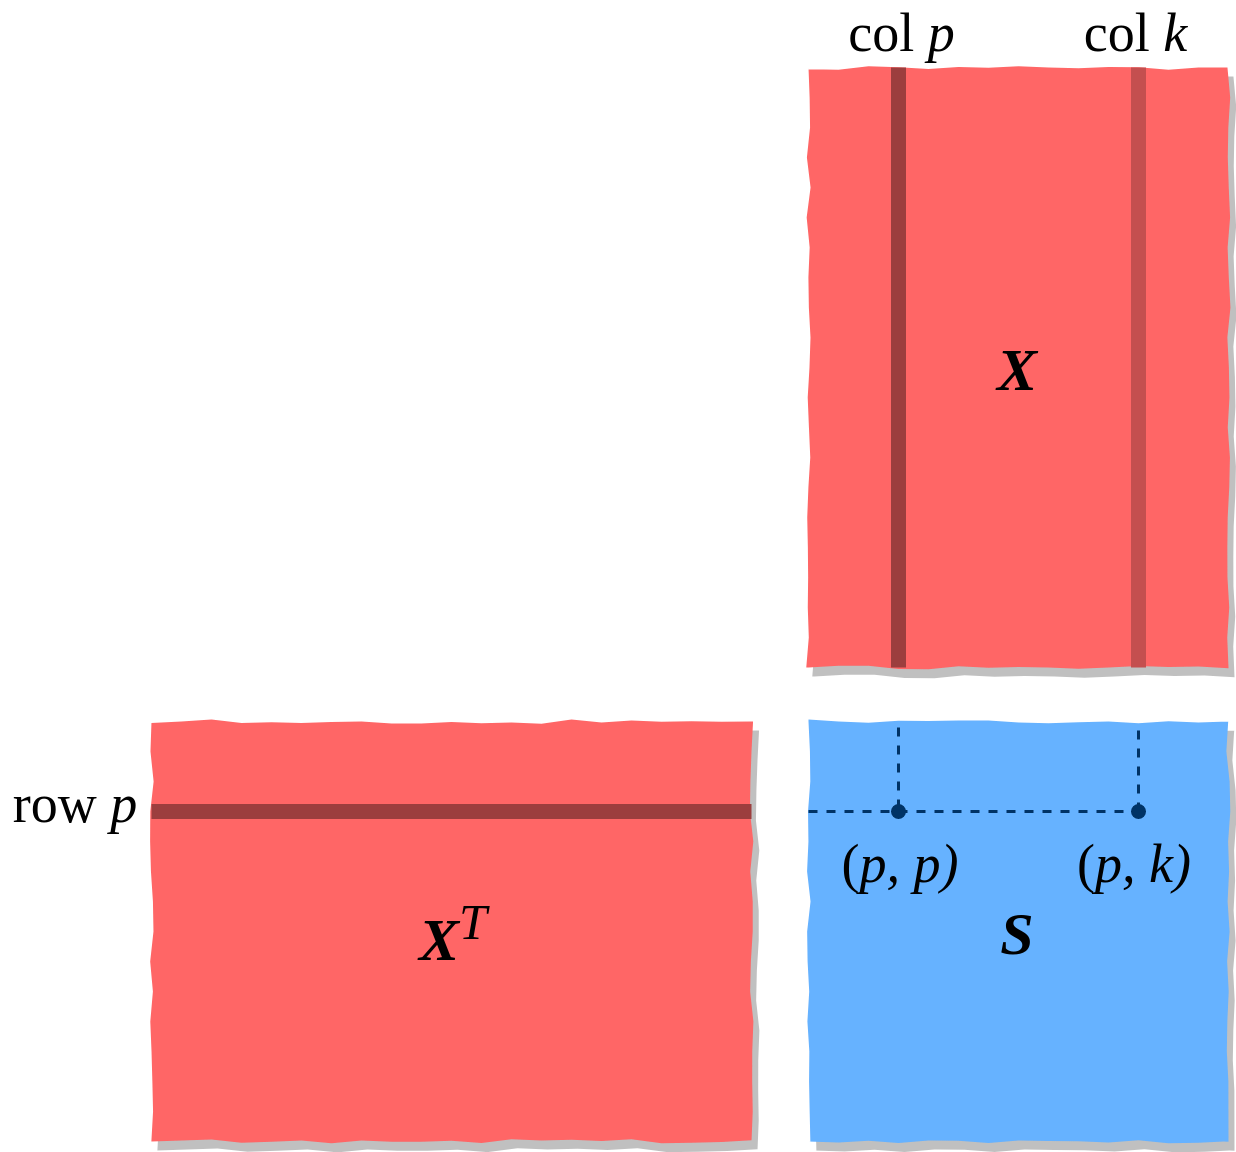
\includegraphics[width=7cm]{cov-matrix.png}
\caption{Covariance matrix $\bm{S}$ graphical interpretation.}
\label{fig:covariance-matrix}
\end{figure}

Notice that an element at position $(p,k)$ inside the covariance matrix has the interpretation of a dot product between a vector formed by the $p$-th row of a matrix $\bm{X}^T$ and the $k$-th column of a matrix $\bm{X}$.
%There is also the factor $\frac{1}{n-1}$ out front, which we discuss in a closer detail in the Appendix \ref{app:B}.

\begin{equation}
s_{p,k} = \frac{1}{n-1} (\bm{x}_p^T \circ \bm{x}_k)
\end{equation}

The similarity with eq.(\ref{eq:covariance-definition}) is now even more evident. Notice that as long as the columns of $\bm{X}$ have been centered, the off-diagonal elements of the covariance matrix have the mathematical meaning of covariance between two variables.

In a case where we multiply row $p$ with column $p$, we get a dot product of a vector with itself:

\begin{equation}
s_{p,p} = \frac{1}{n-1} ( \bm{x}_p^T \circ \bm{x}_p)
\end{equation}

This in turn looks similar to eq.(\ref{eq:variance-definition}) and thus the diagonal elements of the covariance matrix represent the variance of a single variable.

In general, the dot product between two vectors $\bm{x}$ and $\bm{y}$ represents how much vector $\bm{x}$ lays in the direction of vector $\bm{y}$ (and vice versa) - and it is zero when two vectors are perpendicular to each other. This intuition can be carried to the covariance matrix. If any off-diagonal element is non-zero, say element at position $(p,k)$ it means that some information about a $p^{th}$ variable is carried by a $k^{th}$ variable (and vice versa).

\subsection{Properties} \label{sec:covariance-properties}

The covariance matrix is a very special matrix and it is worth pointing out some of its interesting properties that the Principal Component Analysis makes extensive use of.

First of all, any matrix constructed as: $\bm{S} = \bm{C}^T \bm{C}$ (where $\bm{C}$ is any real matrix) is square and symmetric\footnote{the symmetry follows from the symmetry in: $\text{cov}(\bm{x},\bm{y}) = \text{cov}(\bm{y},\bm{x})$.} (the reason for this is easy to see from Fig.\ref{fig:covariance-matrix}). Apart from that, the eigenvalues of such matrix are real and all are at least non-negative - such matrix is called a \textit{positive semidefinite} matrix. In a practical case that we are most interested in, this matrix has got only positive eigenvalues and we call it a \textit{positive definite} matrix.

Another important property is that the eigenvectors of the covariance matrix are orthogonal, which is a very special thing indeed. You may already see some interesting uses for such eigenvectors. One of which could be: they can form a new, $Q$-dimensional coordinate system - a \textit{basis}. Hopefully we are now on the right track to convincing you that such basis can be a very interesting basis.

Finally, the eigenvalues associated with the eigenvectors are ordered in a decreasing order with the first one being the highest. This property becomes very useful for dimensionality reduction.

\subsection{Some remarks}

Interestingly, computing a dot product between two vectors is not the only way to \textit{measure} covariance between variables. This might come as a surprise at first, but think for instance about different ways that we can measure distance. Euclidean distance is just \textit{a} way and not \textit{the} way - other distance metrics exist such as city block or Mahalanobis distance. Everything depends on your use case. The same story can be told about covariance. If up to this point in the tutorial I managed to convince you that computing dot products is how we should populate the covariance matrix then you probably start to wonder: would there be any meaning in doing it differently? Well, here's a brain twister: as long as the resulting covariance matrix is symmetric, we can populate it however we want. In other words, we can generate a \textit{rule} that takes two vectors and gives a scalar as a result. We often call that rule a \textit{covariance function} or a \textit{covariance kernel}. This might give us many advantages, as now we become chefs managing our variables in a data set and we specify how we would like our variables to correlate\footnote{This concept is a basis for formulating a variation of the classical PCA presented here - Kernel PCA.}.

% If you want to explore this subject more, I invite you to check out my other tutorial on Gaussian Process Regression.

\section{PCA workflow}

As you may have already anticipated, the next step in PCA is to perform the eigendecomposition of the covariance matrix:

\begin{equation} \label{eq:eig-dec}
\text{eig}(\bm{S}) = [\bm{A}, \bm{\Lambda}]
\end{equation}



$\bm{A}$ is a matrix of eigenvectors and it is size $(Q \times Q)$. Each eigenvector is called a \textit{principal component} (PC). The principal components are orthogonal (due to properties discussed in \ref{sec:covariance-properties}) and therefore another important property holds: $\bm{A}^T = \bm{A}^{-1}$ (proof\footnote{for orthogonal columns of $\bm{A}$ we have $\bm{A}^T \bm{A} = \bm{I}$. Multiplying both sides by $\bm{A}^{-1}$ we get $(\bm{A}^T \bm{A}) \bm{A}^{-1}= \bm{I}\bm{A}^{-1}$. Since matrix multiplication is associative, we may also perform: $\bm{A}^T (\bm{A} \bm{A}^{-1}) = \bm{A}^{-1}$. From definition of an inverse matrix,  $\bm{A} \bm{A}^{-1} = \bm{I}$, hence: $\bm{A}^T = \bm{A}^{-1}$.}).

The diagonal matrix $\bm{\Lambda}$ of size $(Q \times Q)$ is a matrix of the corresponding eigenvalues.

\begin{figure}[H]
\centering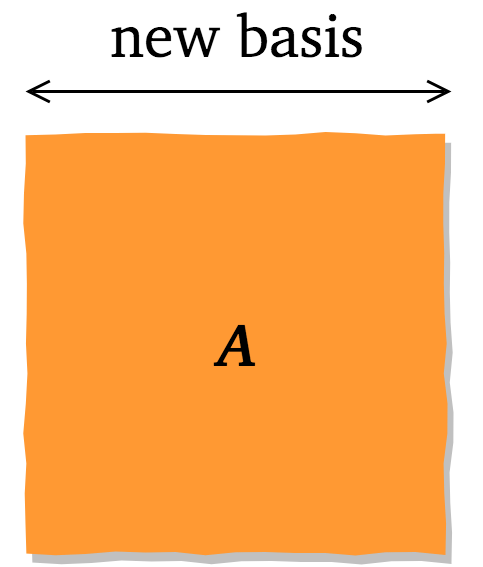
\includegraphics[width=3cm]{new-basis.png}
\caption{Eigenvalues of the covariance matrix form a new orthogonal basis.}
\label{fig:new-basis}
\end{figure}

Given the eigendecomposition of matrix $\bm{S}$, we may state that: 

\begin{equation} \label{eq:eig-dec-cov-matrix}
\bm{S} = \bm{A} \bm{\Lambda} \bm{A}^T
\end{equation}

The principal components form a new basis in which we can represent our data set. We perform a transformation of the original data matrix $\bm{X}$ from the original space to the new space represented by the PCs. This transformation is achieved with the following multiplication:

\begin{equation} \label{eq:data-transform}
\bm{Z} = \bm{X} \bm{A}
\end{equation}

\begin{figure}[H]
\centering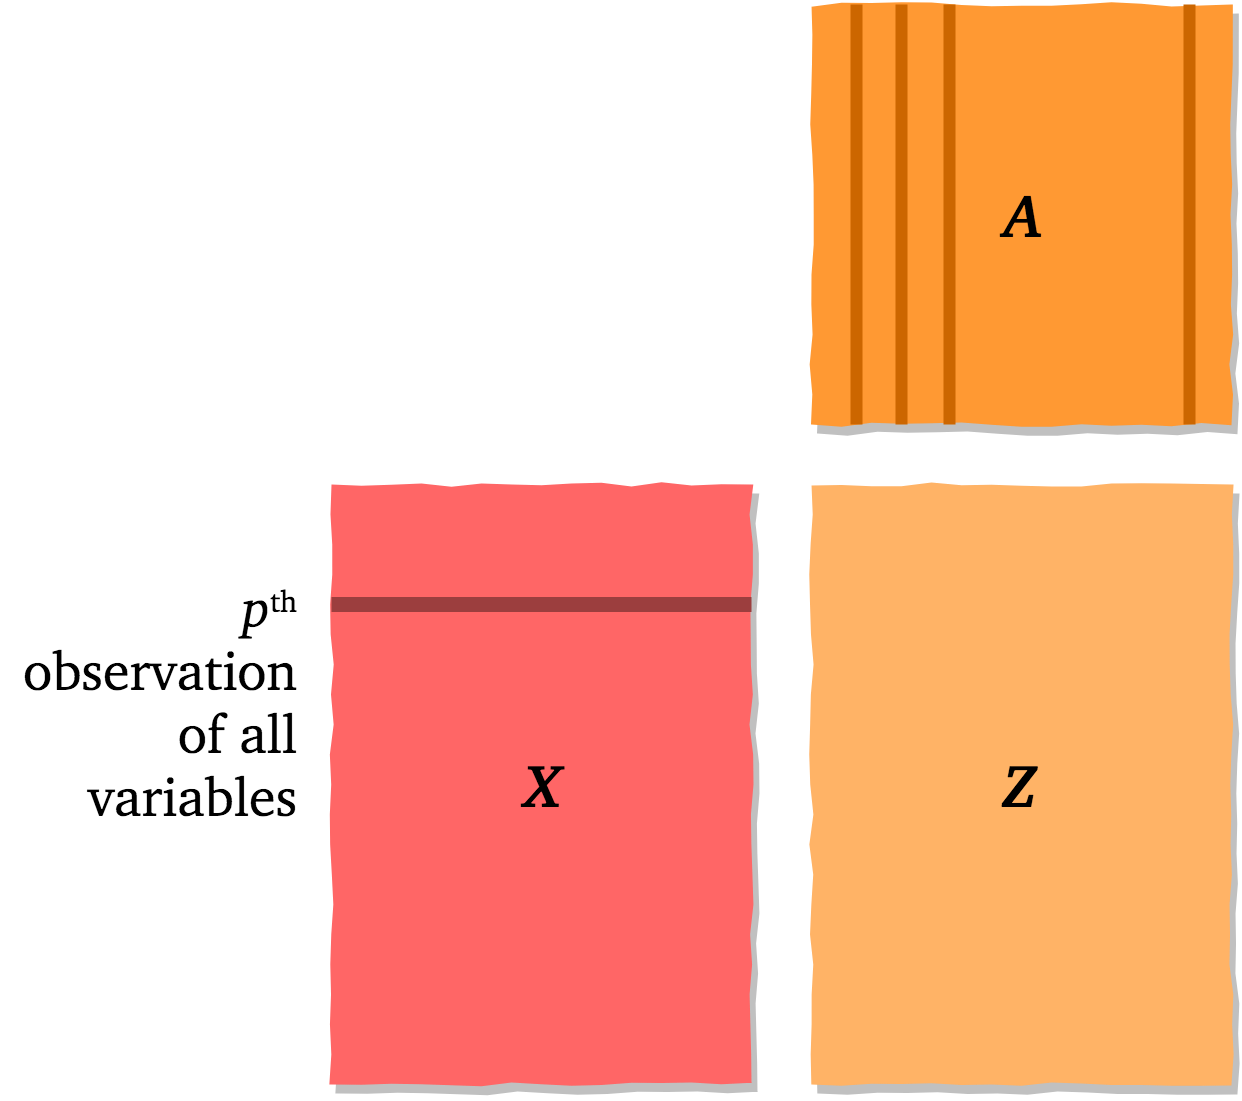
\includegraphics[width=6cm]{data-transformation.png}
\caption{Data transformation to a new basis.}
\label{fig:data-transformation}
\end{figure}

The new matrix $\bm{Z}$ is still our dataset $\bm{X}$ but represented in the basis associated with the matrix $\bm{A}$. It is also called the \textit{PC-scores} matrix, since one may think of every element in this matrix as a "score" that the corresponding element in $\bm{X}$ gets when represented in the new coordinate system after transformation. In the matrix multiplication from eq.(\ref{eq:data-transform}), every variable vector inside $\bm{X}$ gets transformed by the transformation matrix $\bm{A}$ and attains new scores in the basis associated with $\bm{A}$. The new representation of the old variable is now kept in the matrix $\bm{Z}$.



We now approach the dimensionality reduction but first let's obtain the original data set back, given the PC-scores and the transformation matrix:

\begin{equation} \label{eq:X-retrieval}
\bm{X} = \bm{Z} \bm{A}^T
\end{equation}

The above equation is our route back to obtain the original data set in which the PC-scores are projected on the basis associated with a transposed eigenvectors matrix $\bm{A}$ (the fact that $\bm{A}^T = \bm{A}^{-1}$ now appears in all  of its usefulness).

Suppose that we would like to find the approximation of the data matrix $\bm{X}$ with only $q$ principal components (we project the PC-scores onto only $q$ out of $Q$ principal components).

We shrink the transformation matrix $\bm{A}$ to the size $(Q \times q)$ (we only keep $q$ columns of $\bm{A}$). To match the matrix sizes we also need to shrink in size the PC-scores matrix which is originally of size $(n \times Q)$. We will denote these truncated matrices $\bm{A_q}$ and $\bm{Z_q}$ respectively.



Projecting $\bm{Z_q}$ onto the basis $\bm{A_q}^T$ will result in an an approximation of the original data set:

\begin{equation} \label{eq:X-approximation}
\bm{X_q} = \bm{Z_q} \bm{A_q}^T
\end{equation}

It is now worth discussing how good is such approximation. It turns out that $\bm{X_q}$ is the closest rank-$q$ approximation to $\bm{X}$ in terms of three popular norms: $L^2$-norm, Frobenius norm and trace norm (also known as nuclear norm). This is known as the Eckart-Young theorem \cite{eckart-young}.

\begin{figure}[H]
\centering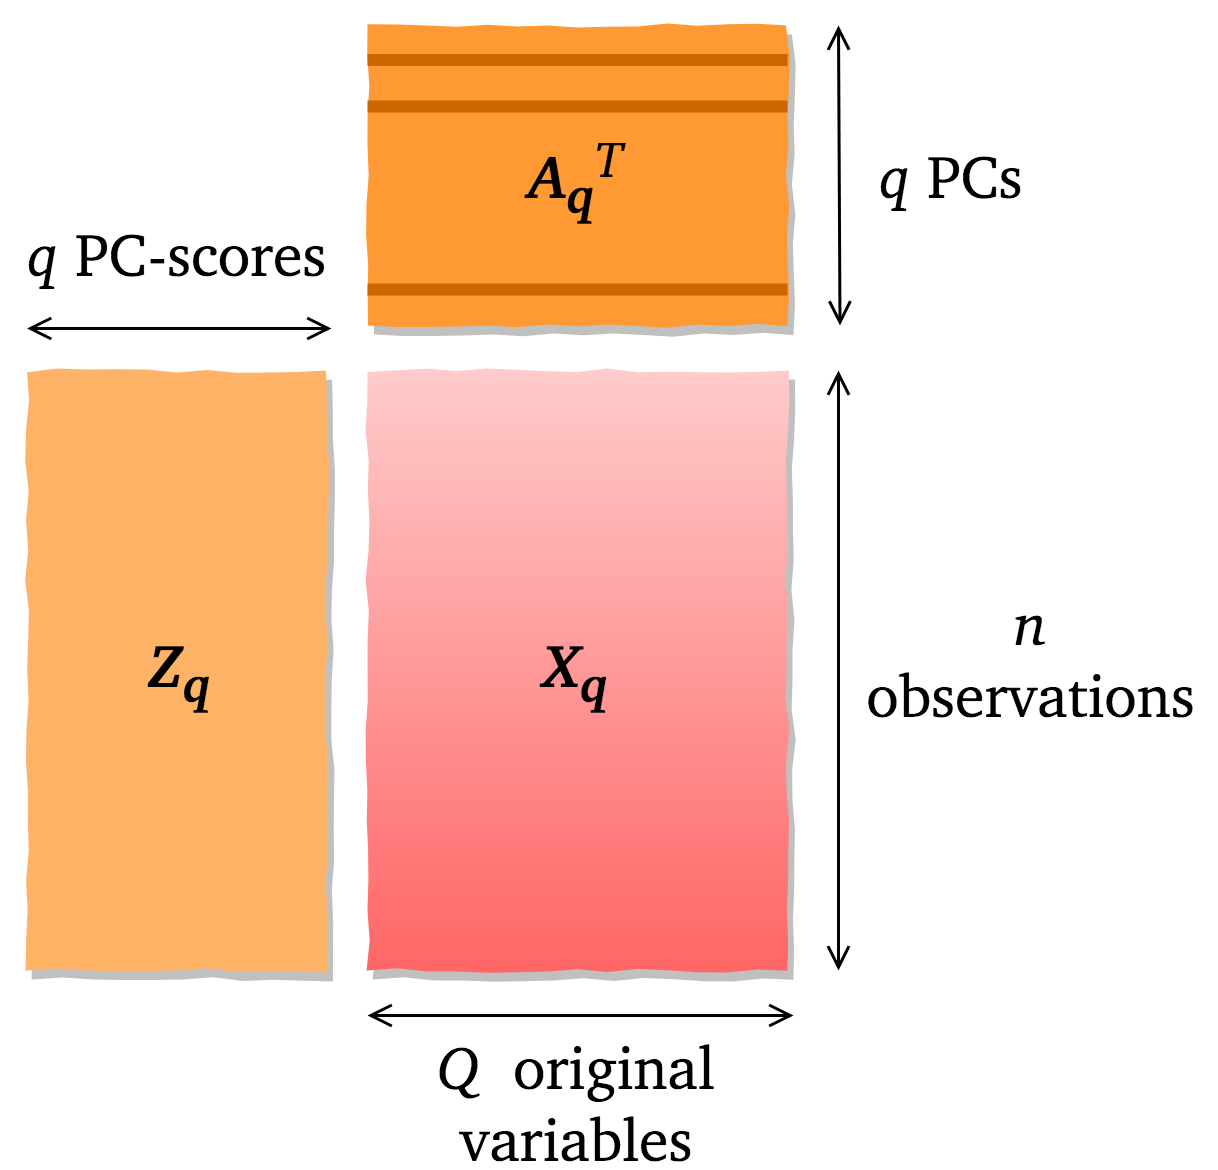
\includegraphics[width=6.1cm]{data-approx.png}
\caption{Data approximation with $q$ PCs.}
\label{fig:data-approx}
\end{figure}

\section{Why eigenvectors?}

In this section we come back to the eq.(\ref{eq:eig-dec}) and answer the question: why are principal components the eigenvectors of a covariance matrix? 

To begin the understanding, let's look at Fig.\ref{fig:PC-scores}. Principal Component Analysis aims to find a new, transformed data set $\bm{Z}$ such that if we computed a new covariance matrix in such a way:

\begin{equation}
\bm{S_Z} =  \frac{1}{n-1} \bm{Z}^T \bm{Z}
\end{equation}

the variances (the elements on the diagonal) are maximized and the covariances (the off-diagonal elements) are zero. This means that no more information about any column of $\bm{Z}$ is carried by any other column of $\bm{Z}$. This removes the redundancy of information that could have been present in the original data set $\bm{X}$; each column of $\bm{Z}$ now contributes to a "unique" piece of information that cannot be found in any other column of $\bm{Z}$. In other words:

\,\,

\textbf{The goal of PCA is to diagonalize the new covariance matrix $\bm{S_Z}$.}

\,\,

As a "template" for a diagonal matrix, PCA uses a diagonal matrix that is easily available (and which we have already produced!) - the matrix of eigenvalues $\bm{\Lambda}$. We will now ask ourselves: how do we need to construct $\bm{Z}$, so that the matrix $\bm{S_Z} = \bm{\Lambda}$?

We find $\bm{Z}$ through a series of transformations in which we combine eq.(\ref{eq:eig-dec-cov-matrix}) with eq.(\ref{eq:cov-matrix}):

\begin{equation}
\bm{A} \bm{\Lambda} \bm{A}^T =  \frac{1}{n-1} \bm{X}^T \bm{X} \,\, \Big/ \bm{A}^T \times
\end{equation}

\begin{equation}
\bm{A}^T \bm{A} \bm{\Lambda} \bm{A}^T =  \frac{1}{n-1} \bm{A}^T  \bm{X}^T \bm{X} \,\, \Big/ \times \bm{A}
\end{equation}

\begin{equation}
\bm{A}^T \bm{A} \bm{\Lambda} \bm{A}^T \bm{A} =  \frac{1}{n-1} \bm{A}^T  \bm{X}^T \bm{X} \bm{A}
\end{equation}

\begin{equation}
\bm{I} \bm{\Lambda} \bm{I} =  \frac{1}{n-1} \bm{A}^T  \bm{X}^T \bm{X} \bm{A}
\end{equation}

\begin{equation}
\bm{S_Z}  = \bm{\Lambda} = \frac{1}{n-1} \bm{A}^T  \bm{X}^T \bm{X} \bm{A}
\end{equation}

It is thus visible, that if we chose $\bm{Z} = \bm{X} \bm{A}$, the product $\bm{Z}^T \bm{Z}$ give a diagonal matrix.\footnote{Note here that if $\bm{Z} = \bm{X} \bm{A}$, then $\bm{Z}^T = (\bm{X} \bm{A})^T = \bm{A}^T \bm{X}^T$.}

\begin{figure}[H]
\centering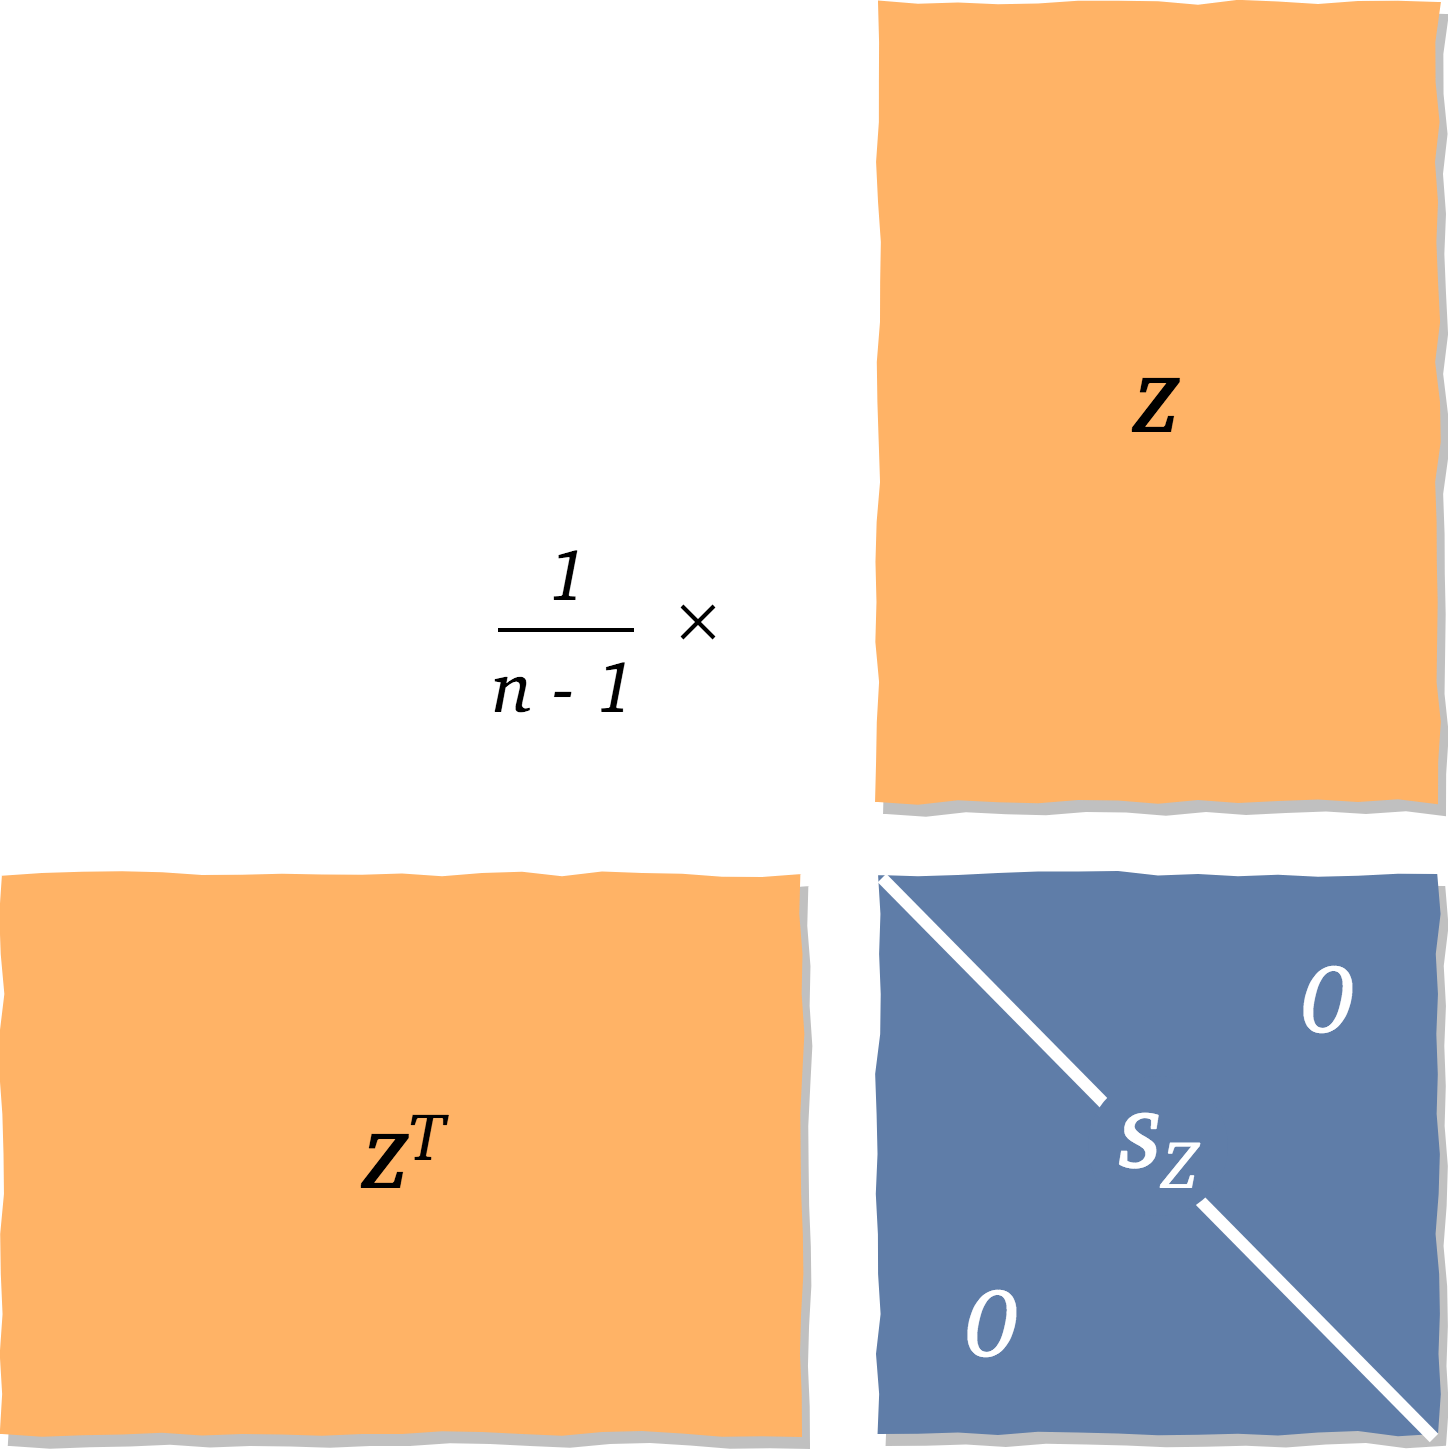
\includegraphics[width=6cm]{PC-scores.png}
\caption{New transformed data set $\bm{Z}$ and its diagonal covariance matrix $\bm{S_Z}$.}
\label{fig:PC-scores}
\end{figure}

There is one more great thing that PCA achieves: the elements on the diagonal of the new covariance matrix are maximized. PCA achieves both things at the same time: it diagonalizes the new covariance matrix and it makes the diagonal elements maximum possible.

So in fact, we should say:

\,\,

\textbf{The goal of PCA is to diagonalize the new covariance matrix $\bm{S_Z}$ and maximize the elements on the diagonal.}

\,\,

Hopefully you could now see for yourself that the basis associated with the eigenvectors of the covariance matrix is a very interesting basis! It lets us diagonalize the product $\bm{Z}^T \bm{Z}$ and it orders the PC-scores from the most to the least \textit{informative} ones.

%\section{Eigenvalues as energy}
%
%You may sometimes encounter the following statement in the literature: the eigenvalues in PCA represent the energy contributions of each of the Principal Components. The energy here is considered in a physical sense, so that since the PCs are ordered, the first ones are said to carry most of the energy, which in mathematical terms was previously treated in terms of variance. Variance and energy can be encountered as terms used interchangeably. How do we know that the eigenvalues associated to PCs can be viewed that way?
%
%In order to understand this, let's introduce a measure called \textit{inertia}, that can be computed for any vector. We would like that measure to capture the amount of             carried by the elements of that vector, on purely numerical grounds.



%\section{How it all links together}
%
%Hopefully by now the steps of PCA begin to look connected. In fact, at least to my eye, PCA  technique seems like a "series of fortunate events" that makes a very effective use of a few popular concepts from linear algebra. 
%
%
%
%\section{Special topics}
%
%\subsection{PCA on a rank-deficient matrix}
%
%It is interesting to think about what PCA accomplishes on a rank-deficient matrix - one where rank $r$ is smaller than $Q$. Since PCA would produce $Q$ orthogonal eigenvectors one might ask: is PCA creating additional dimensions beyond the original $r$ ones then?
%
%It is reasonable to expect that the eigenvalues associated to such non-existent dimensions will be zero since there is zero variance on those dimensions in the original data set $\bm{X}$. So one way to account for the original $r$ dimensions in the data set is for PCA to compute only $r$ non-zero eigenvalues.
%
%But what about the approximation of the data $\bm{X_q} = \bm{Z_q} \bm{A_q}^T$ when $q=Q$? What is the rank of the reconstructed $\bm{X_Q}$?
%
%
%\subsection{Rotation of PCs}



\newpage

\section*{Appendix}

\appendix

\section{Visualizing PCA with Python}

\subsection{Plotting the workflow}\label{sec:pca-workflow}

We will now go on to visualizing on an artificial 2D data set every step of PCA. We will use the \pythoninline{PCA} function from a Python library \pythoninline{sklearn.decompositions}. The full code can be accessed in the GitHub repository. Here, we will only recall elements of that code that are for performing PCA.

We create the \pythoninline{Dataset} (the equivalent of $\bm{X}$) as follows:

\begin{python}
import numpy as np
Np = 100
x = np.linspace(3, 6, Np)
y = 0.8*x + 1*np.random.rand(Np)
Dataset = np.column_stack((x, y))
\end{python}

Let's assume that the first column of this data set are realizations of the first variable $x$ and the second column are realizations of the second variable $y$.

The two variables $x$ and $y$ span two dimensional space but the data set exhibits a low-dimensional structure which is easily visible to the eye just by looking at the Fig.\ref{fig:python-raw-data}. We already see that the data seems to be spread along some linear function. Perhaps changing the basis to a basis associated with this linear function will be a more effective representation by our data set? Note here also, that for multidimensional data sets "seeing" such data structures is no longer possible (as it still is in 2-D or 3D). We need to rely on the dimensionality reduction technique that we chose to find this low-dimensional structure for us.

\begin{figure}[H]
\centering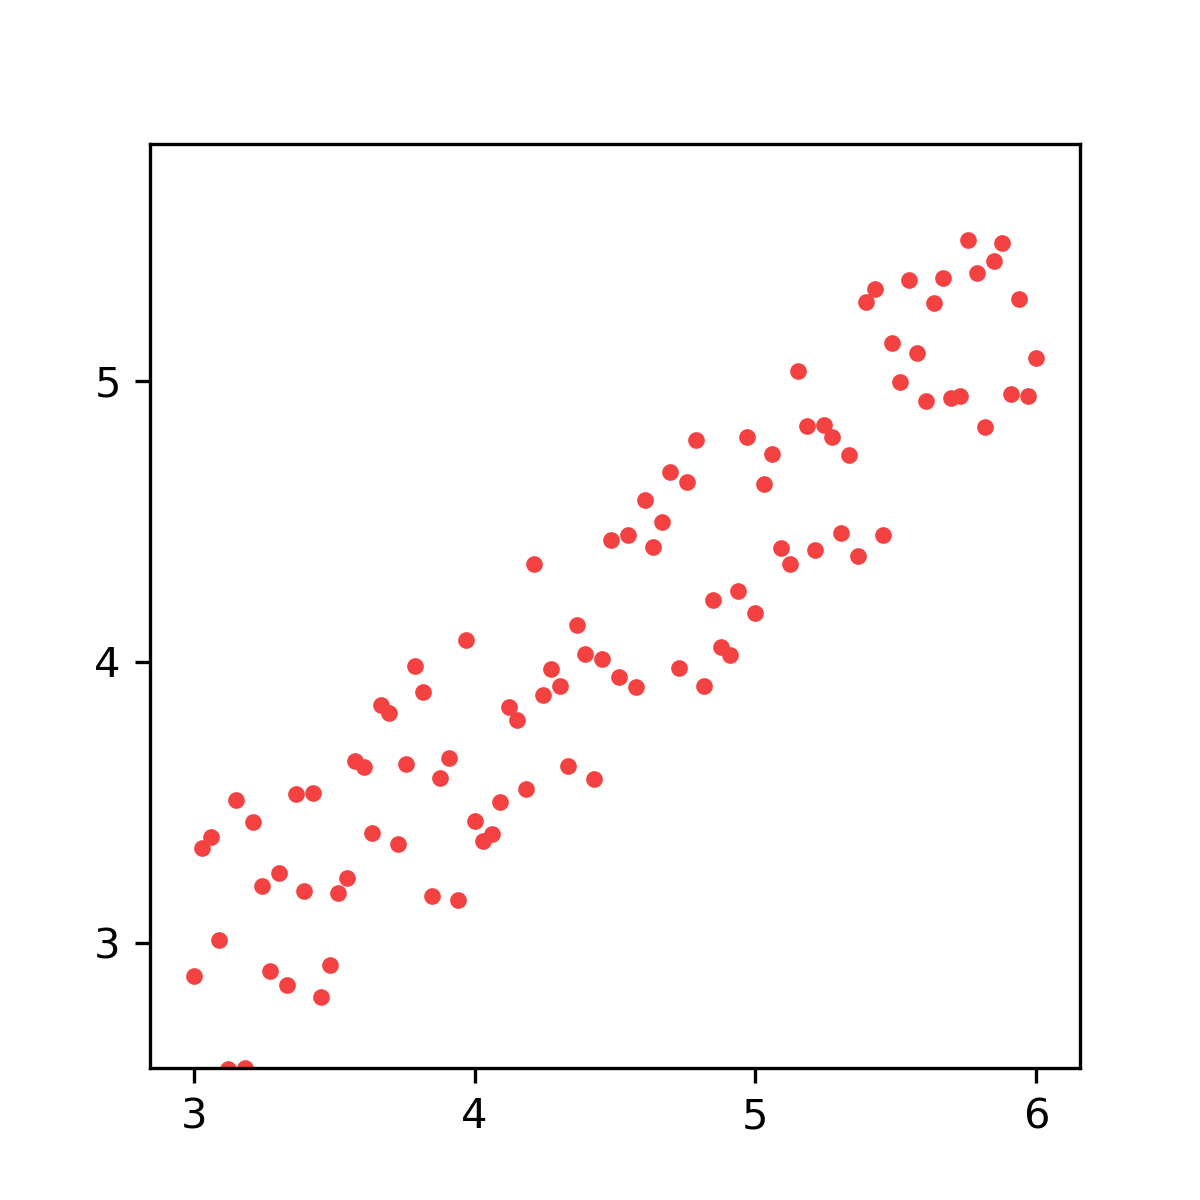
\includegraphics[width=6cm]{python-raw-data.png}
\caption{Raw data set.}
\label{fig:python-raw-data}
\end{figure}

We center the data set, which simply moves the center of the cloud of points to the origin of the coordinate system. If necessary, data set would also be scaled to allow for even comparison of the two variables.

\begin{python}
Dataset_mean = np.mean(Dataset, axis=0)
Dataset_proc = Dataset - Dataset_mean
\end{python}

\begin{figure}[H]
\centering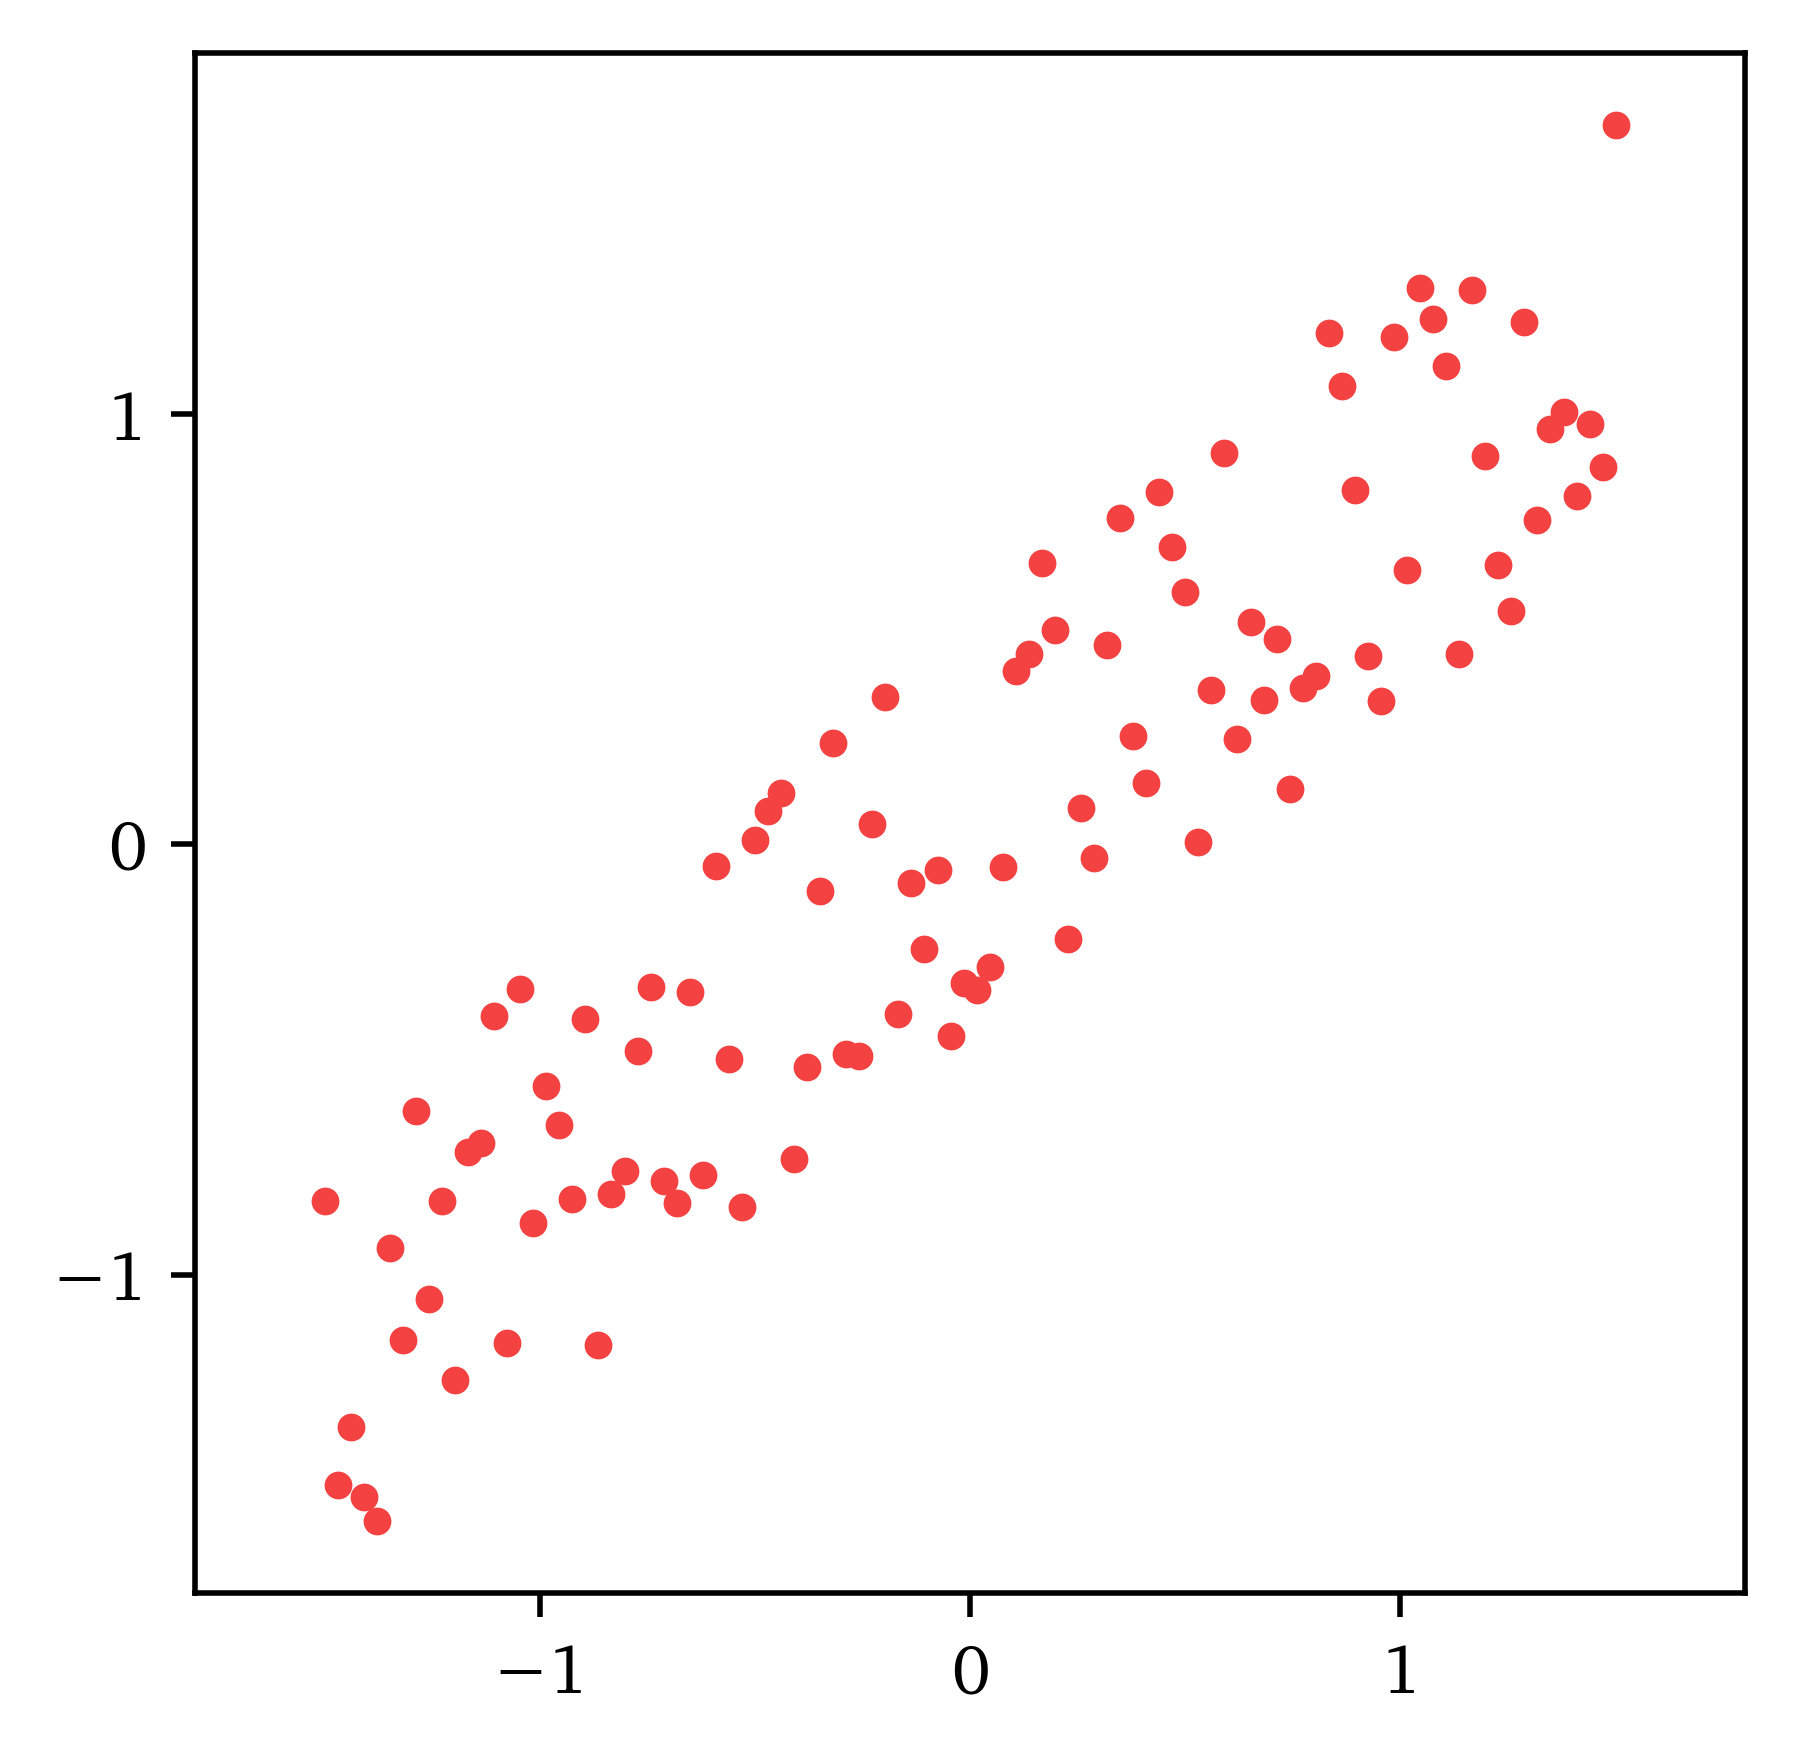
\includegraphics[width=6cm]{python-data-centered.png}
\caption{Data set centered.}
\label{fig:python-raw-data-centered}
\end{figure}

Next, PCA is performed on the dataset and the eigenvectors (the Principal Components) \pythoninline{PCs} are found, with the corresponding eigenvalues \pythoninline{eigvals}.

\begin{python}
from sklearn.decomposition import PCA
pca = PCA()
pca.fit(Dataset)

eigvals = pca.explained_variance_ratio_
PCs = pca.components_
PCscores = pca.transform(Dataset)
\end{python}

In the above code, we create an object \pythoninline{pca} of class \pythoninline{PCA}. We train the model with our \pythoninline{Dataset} using the \pythoninline{fit} function. 

The eigenvectors are plotted on the data set in Fig.\ref{fig:python-PCs}. Their lengths are proportional to their corresponding eigenvalue. Notice that PCA was able to find the direction of the largest variance in the data marked by the direction of the first, longest Principal Component. The second PC is perpendicular to the first one.

\begin{figure}[H]
\centering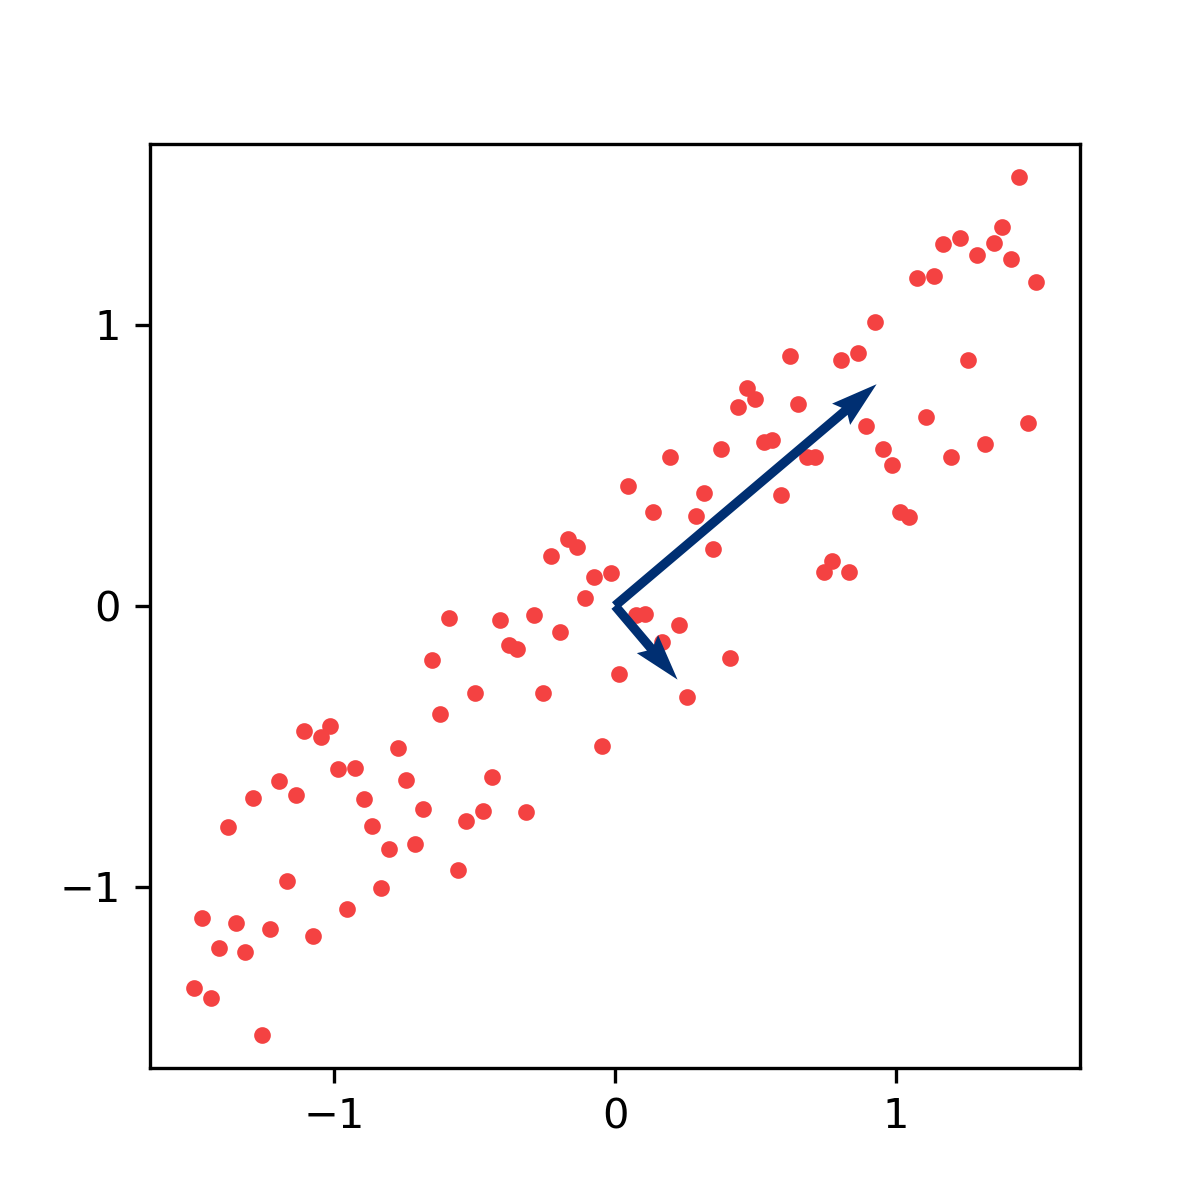
\includegraphics[width=6cm]{python-PCs.png}
\caption{Data set with principal components.}
\label{fig:python-PCs}
\end{figure}

We also compute the transformed data set \pythoninline{PCscores} represented in the basis associated with the obtained \pythoninline{PCs}.
 
\begin{figure}[H]
\centering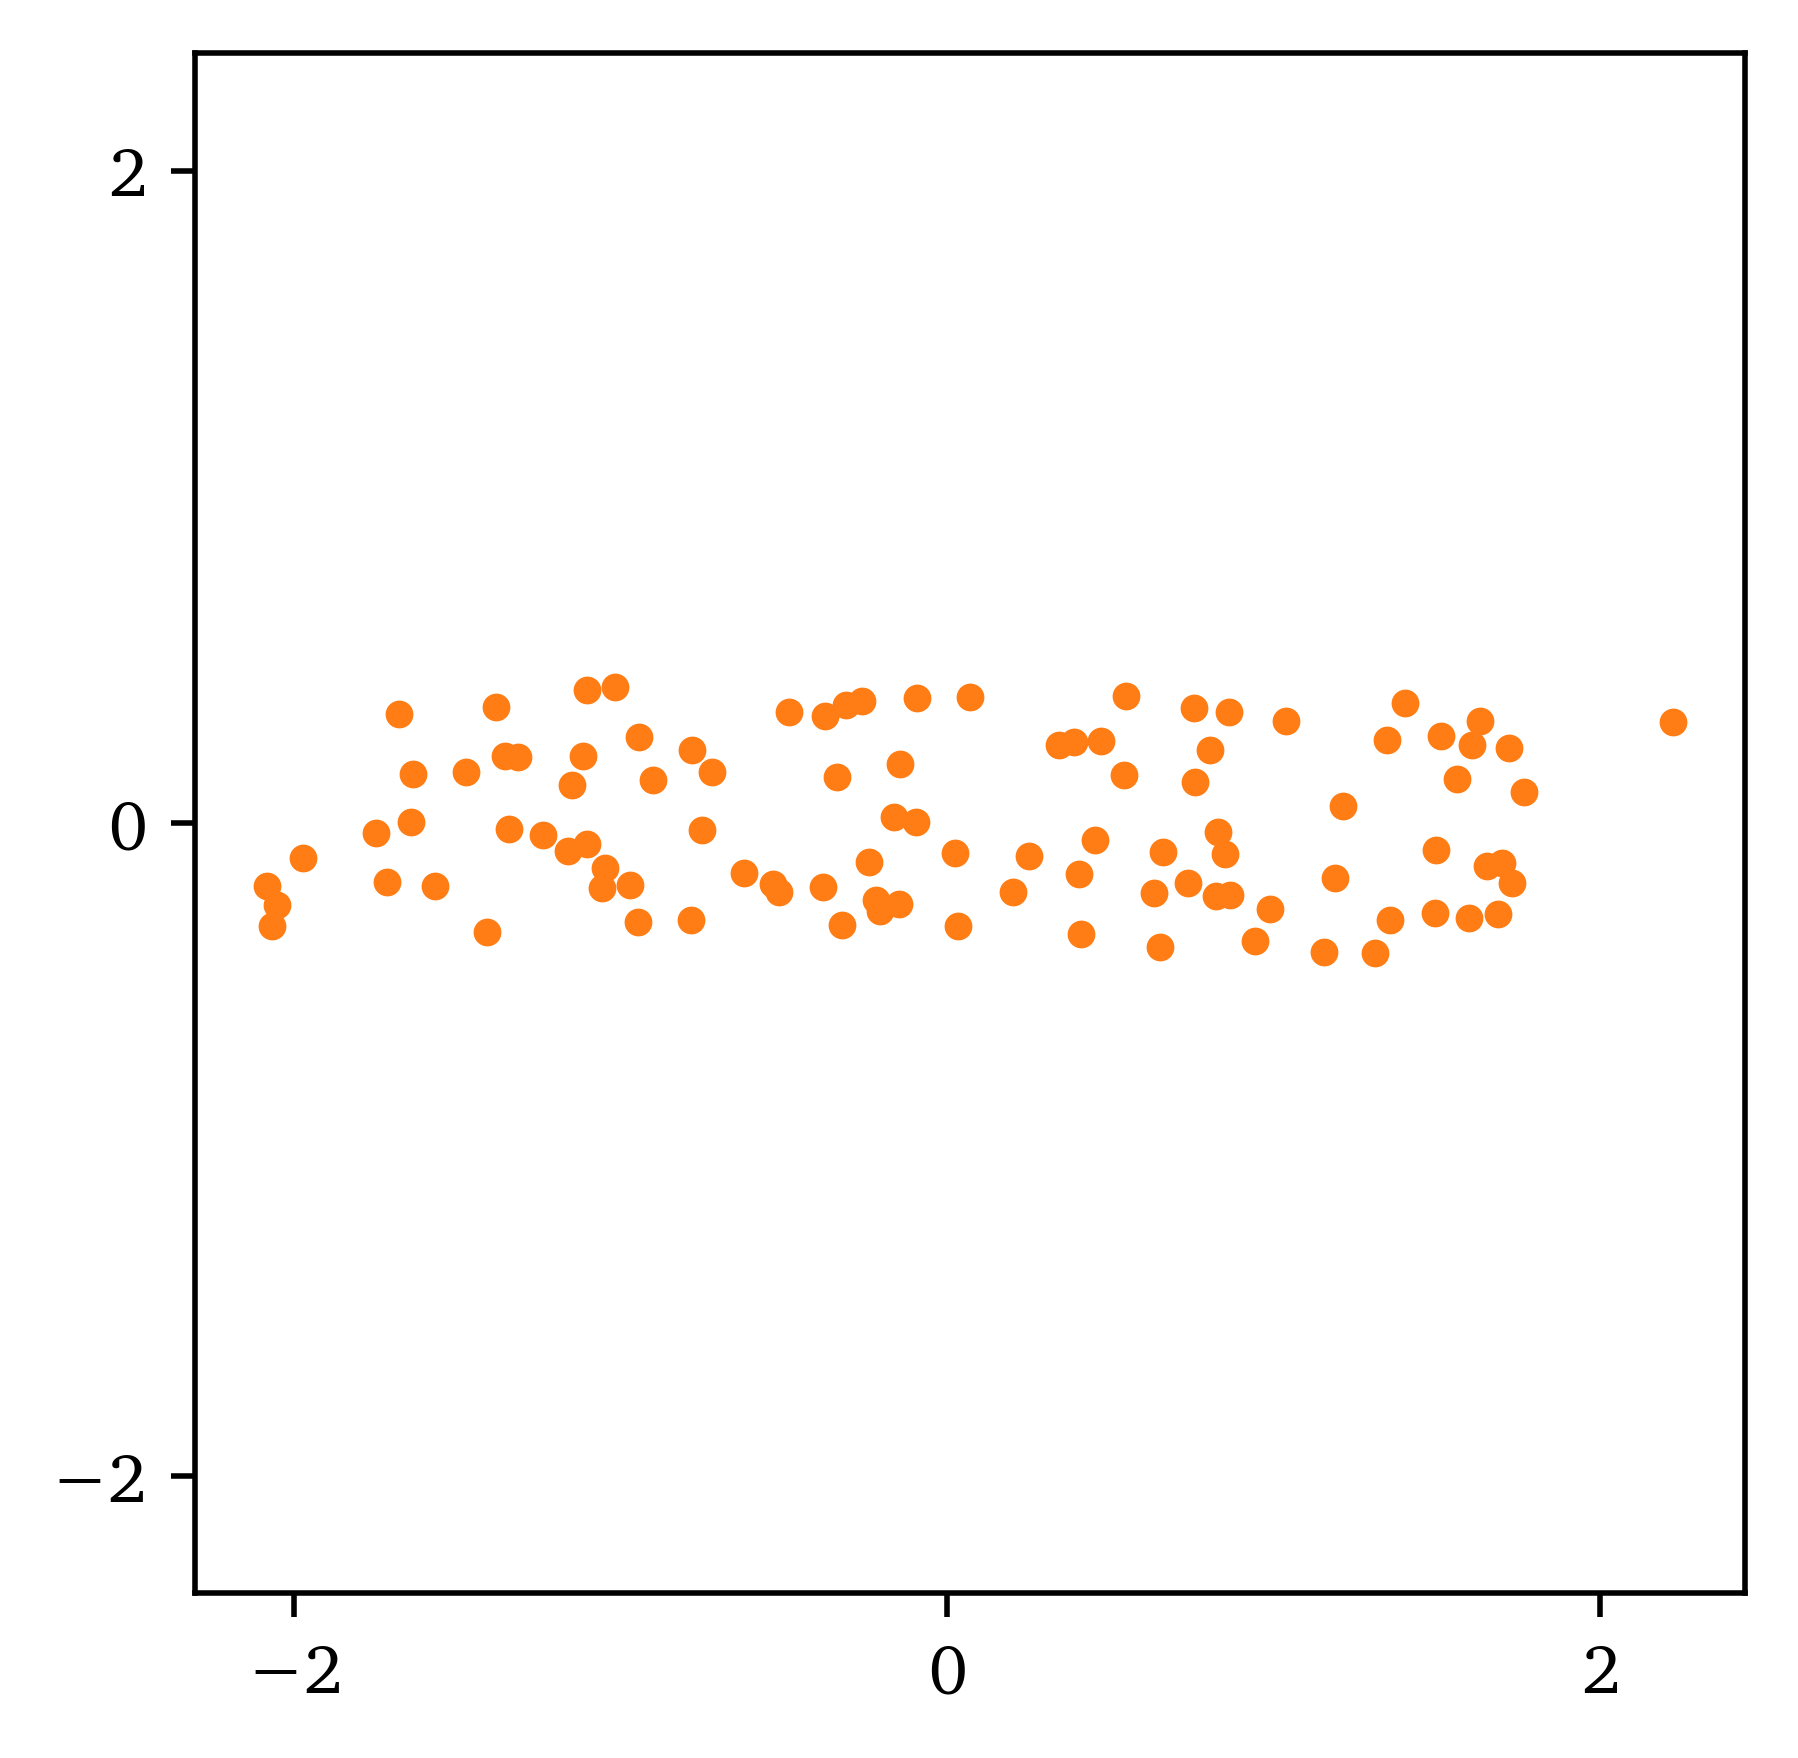
\includegraphics[width=6cm]{python-PC-scores.png}
\caption{PC-scores.}
\label{fig:python-PC-scores}
\end{figure}

Next, the PC-scores can be projected on the first PC, to reduce the dimensionality - from two dimensions to one. The data representation from Fig.\ref{fig:python-data-projection} can be viewed as the "scores" each data point would attain it represented on 1-dimensional structure associated with the first Principal Component.

\begin{python}
q = 1
Dataset_projected = np.dot(Dataset_proc,
np.transpose(pca.components_[:q,:]))
\end{python}

\begin{figure}[H]
\centering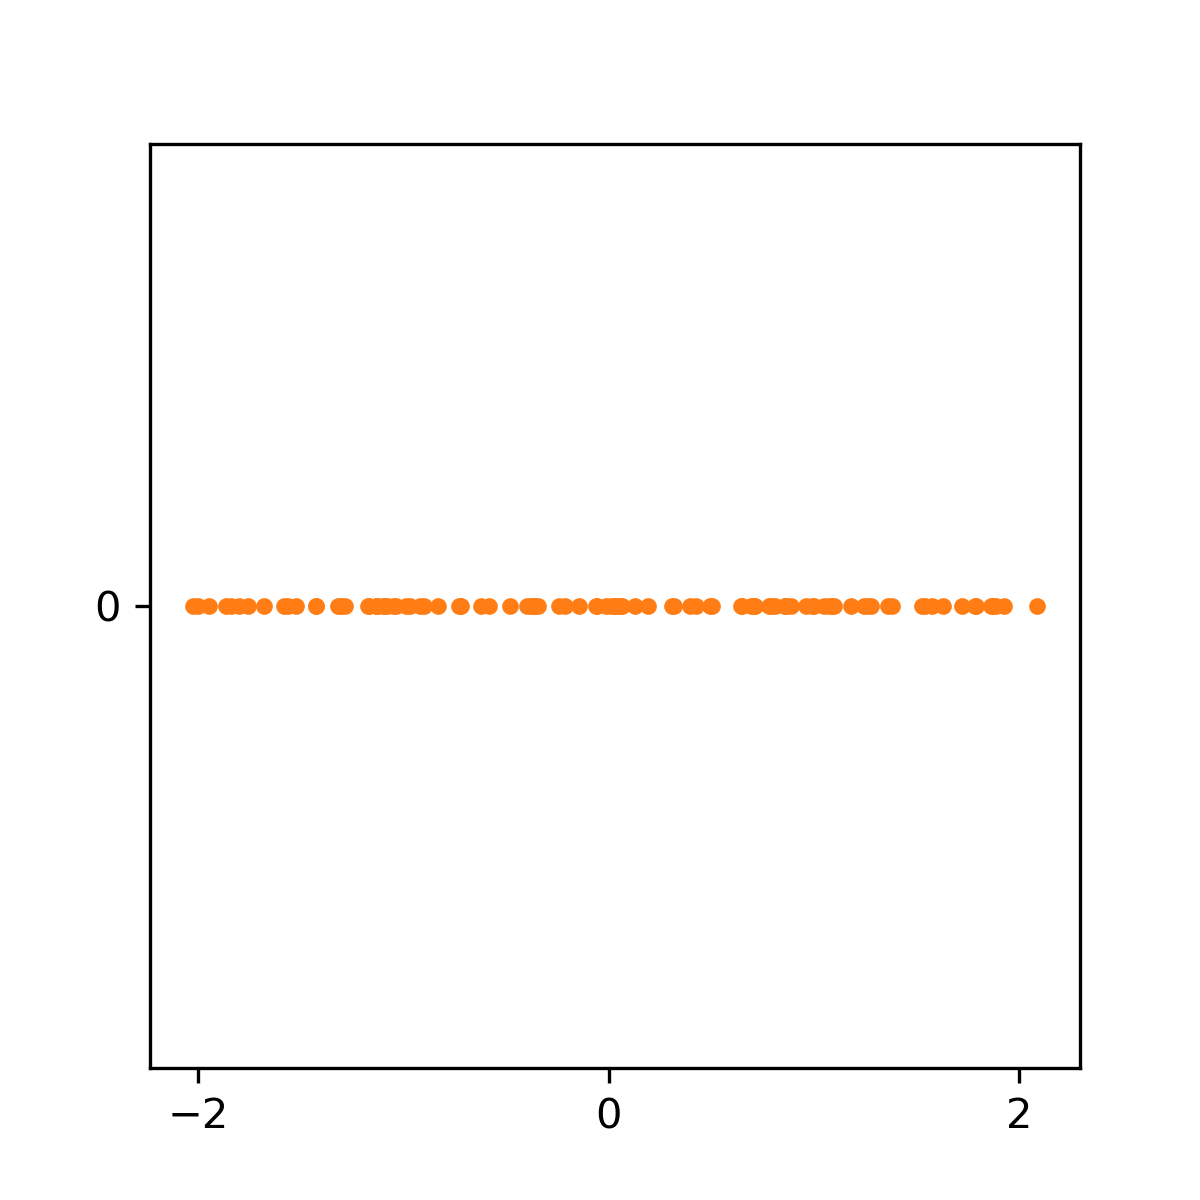
\includegraphics[width=6cm]{python-data-projection.png}
\caption{Data projection on lower dimension.}
\label{fig:python-data-projection}
\end{figure}

We reconstruct the original data set from the reduced space. This represents going back from the 1-dimensional space to the original dimensions. The mean of the data set is added back to undo the data centering.

\begin{python}
Dataset_approx = 
np.dot(pca.transform(Dataset)[:,:q], 
pca.components_[:q,:]) + Dataset_mean
\end{python}

\begin{figure}[H]
\centering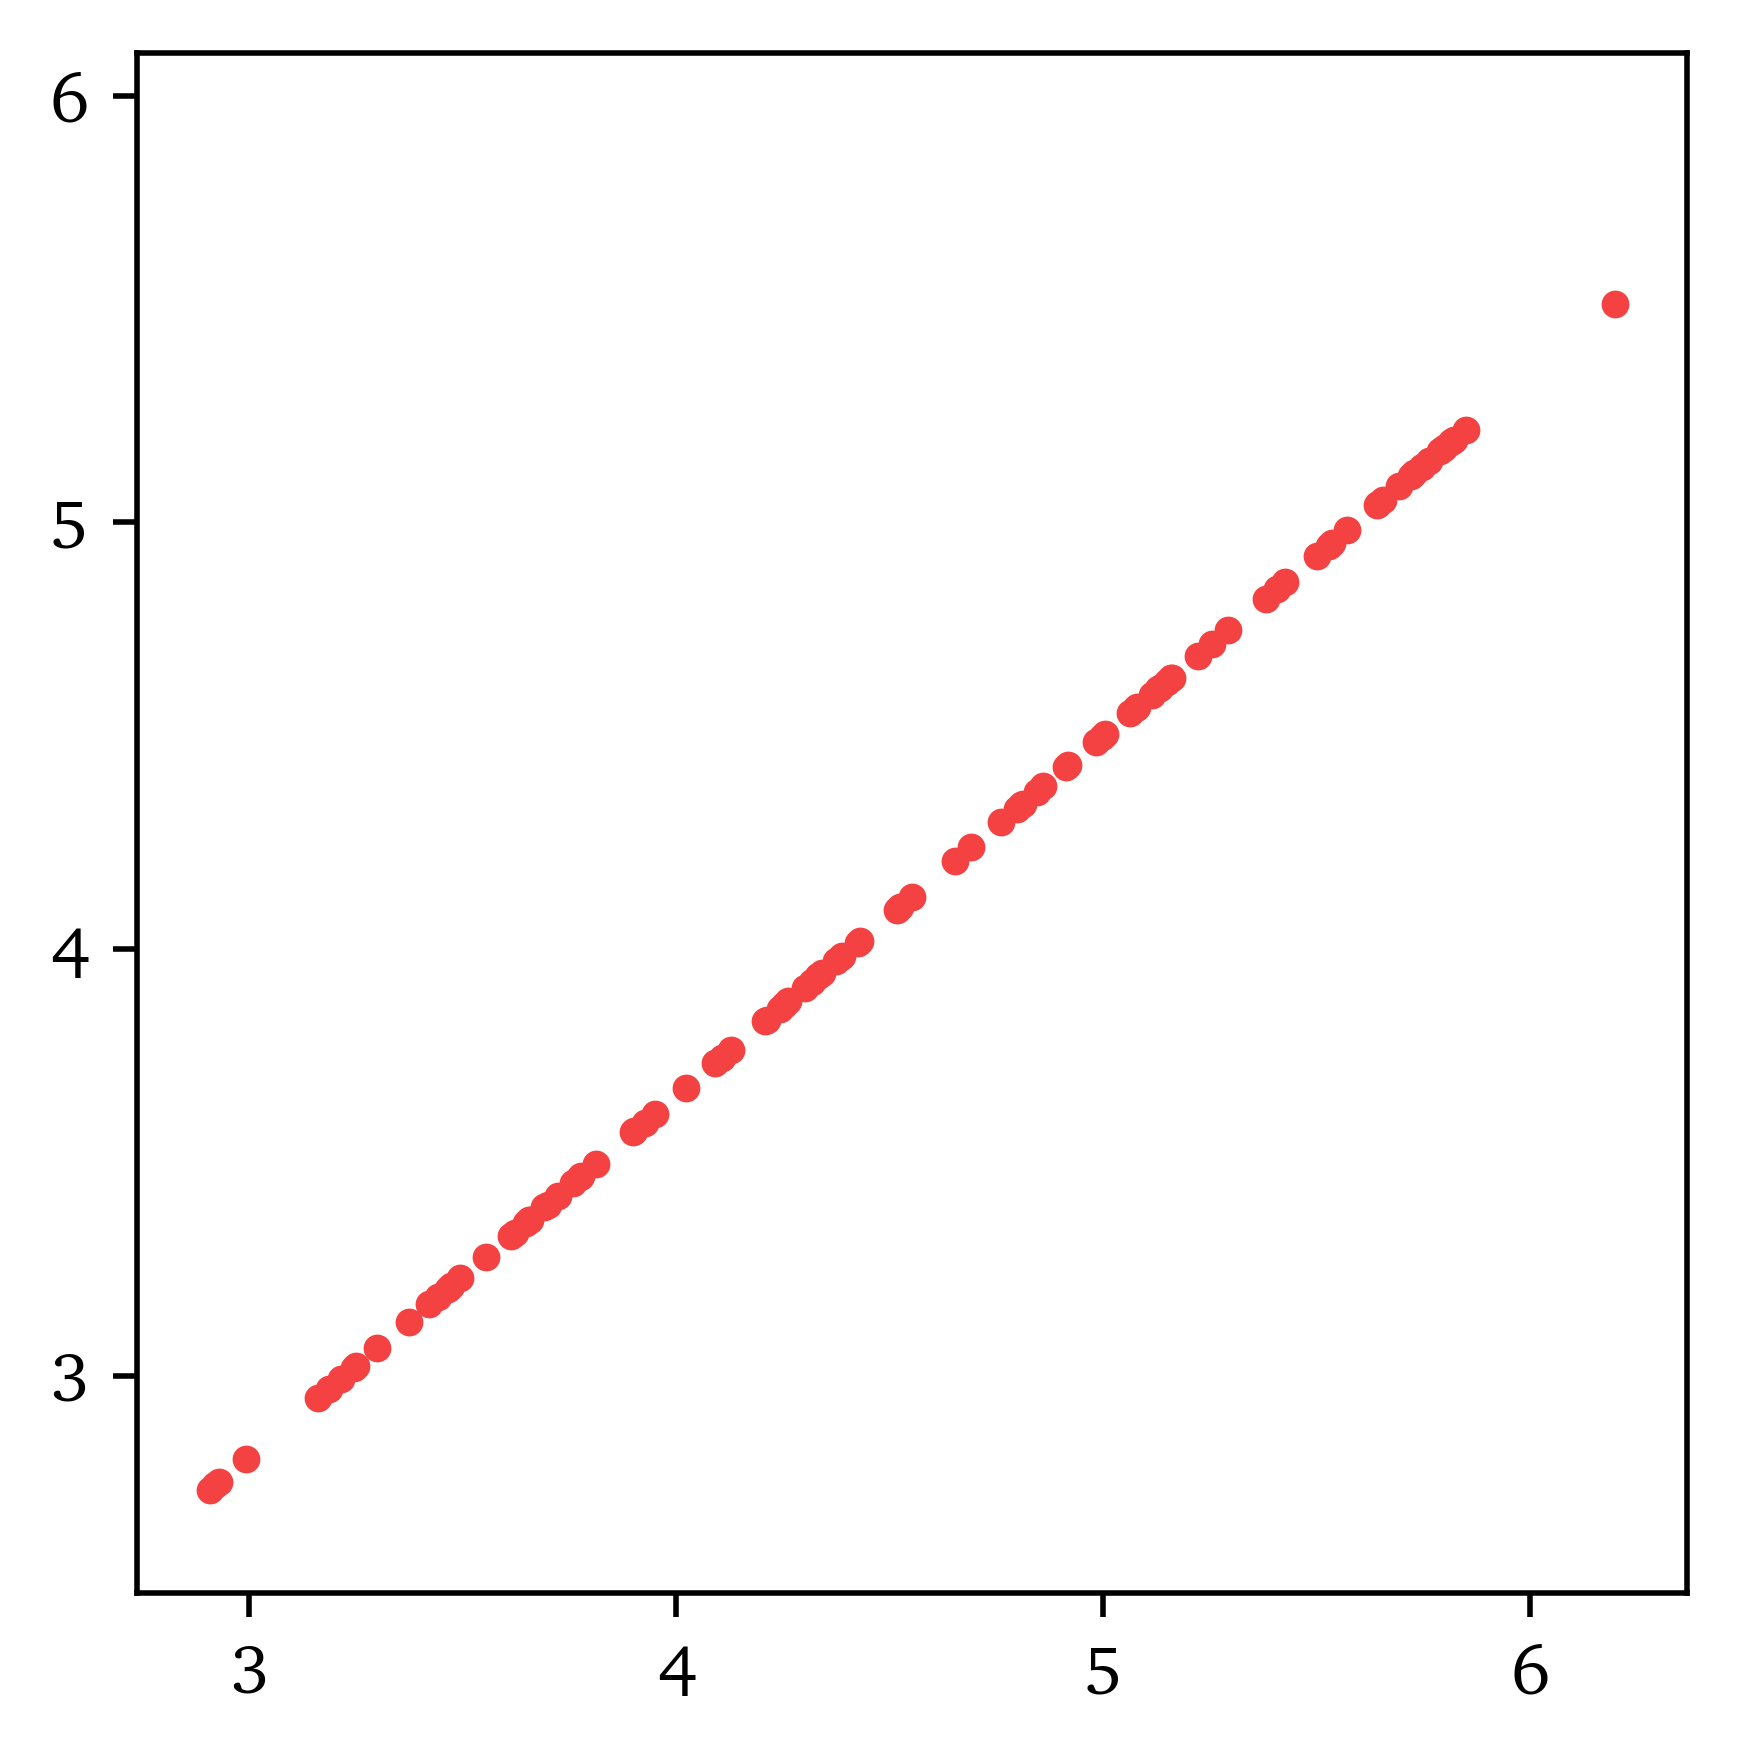
\includegraphics[width=6cm]{python-data-approximation.png}
\caption{Data approximation with $q = 1$.}
\label{fig:python-data-approximation}
\end{figure}

\subsection{Low-rank approximations}

We perform PCA on three artificially generated matrices of size $(10 \times 6)$: a \textbf{random} matrix which is populated by random floats in the range 0-1 and a \textbf{semi-structured} and \textbf{structured} matrices whose elements are also in the range 0-1 but were populated so that there is an increasing level of structure that was judged visually. These matrices are presented in Fig.\ref{fig:matrices}.

\begin{figure}[H]
\begin{subfigure}[t]{.15\textwidth}
\centering

\includegraphics[scale=.2]{DWGs/random-matrix-original.png}
\caption{ }
\end{subfigure}
\begin{subfigure}[t]{.15\textwidth}
\centering
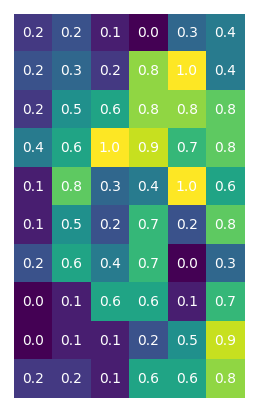
\includegraphics[scale=.2]{DWGs/semi-structured-matrix-original.png}
\caption{ }
\end{subfigure}
\begin{subfigure}[t]{.15\textwidth}
\centering

\includegraphics[scale=.2]{DWGs/structured-matrix-original.png}
\caption{ }
\end{subfigure}
\caption{Original data matrices: (a) random matrix, (b) semi-structured matrix, (c) structured matrix.}
\label{fig:matrices}
\end{figure}

The visual judgment of the level of imposed "structure" is quite objective in this exercise but the aim was to group the elements of high numerical value (most yellow) in a single region of the matrix and elements of low numerical value (most purple) in other regions of the matrix.

The level of the imposed structure can also be observed quantitatively after performing PCA from the eigenvalue distribution, presented in Fig.\ref{fig:eigenvalues}. The structured matrix has got the strongest decaying behaviour which suggest that the matrix can be approximated by relatively low number of modes and hence exhibits the strongest low-rank structure. The first PC is expected to carry 80\% of the total variance in the structured data matrix.

\begin{figure}[H]
\centering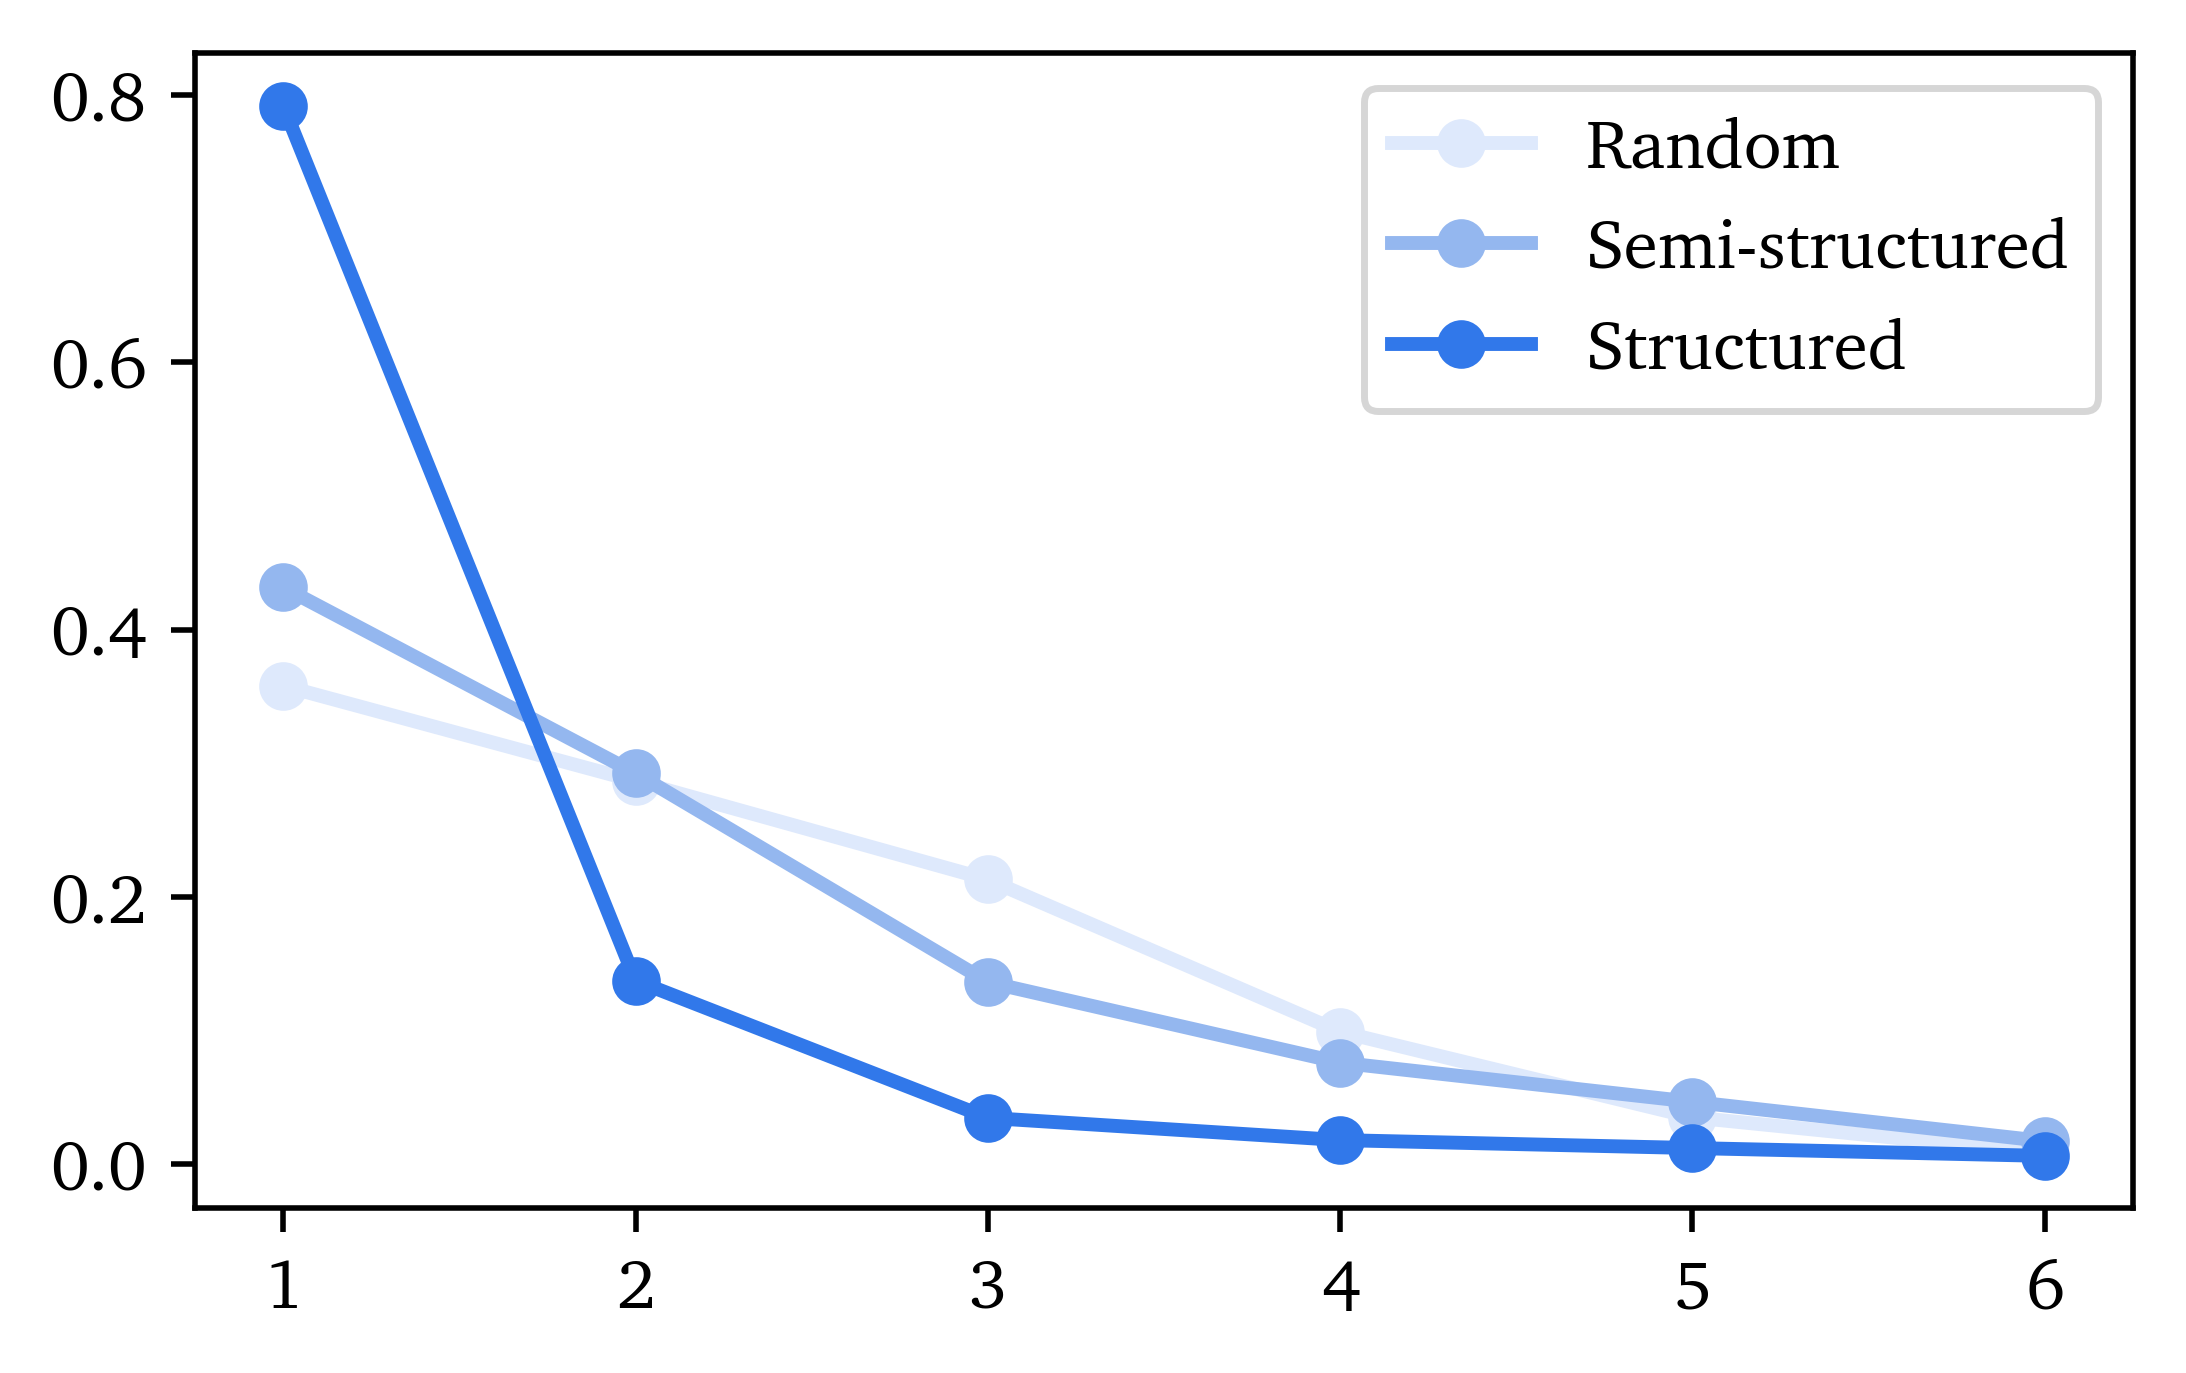
\includegraphics[width=7cm]{DWGs/matrix-reconstruction-eigenvalues-comparison.png}
\caption{Eigenvalue distribution after performing PCA on original data matrices.}			
\label{fig:eigenvalues}
\end{figure}

We reconstruct the original data matrices using a certain number $q$ of PC-scores and corresponding PCs. Using the Matlab notation we may write the approximation as:

\begin{equation} \label{eq:data-set-approximation}
\bm{D}_{\text{app}} = \text{PC-scores}(:,1:q) \cdot \text{PCs}^T(1:q,:) + \bm{D}_{\text{mean}}
\end{equation}

which is equivalent to eq.(\ref{eq:X-approximation}) and to the Python approximation presented in Sec.\ref{sec:pca-workflow}.

The above multiplication is presented in three cases in Fig.\ref{fig:matrices-reconstruction-1}. We can see a rank-1 approximation of the original matrices using the $1^{st}$ Principal Component found by PCA. The vectors $(10 \times 1)$ represent the PC-scores and the vectors $(1 \times 6)$ represent the PCs.

What can be seen visually is that for the semi-structured and structured matrix the low numerical value region is clearly separated. For the random matrix, only few regions of lowest and highest numerical values are recovered in the rank-1 approximation.

%\begin{figure}[H]
%\centering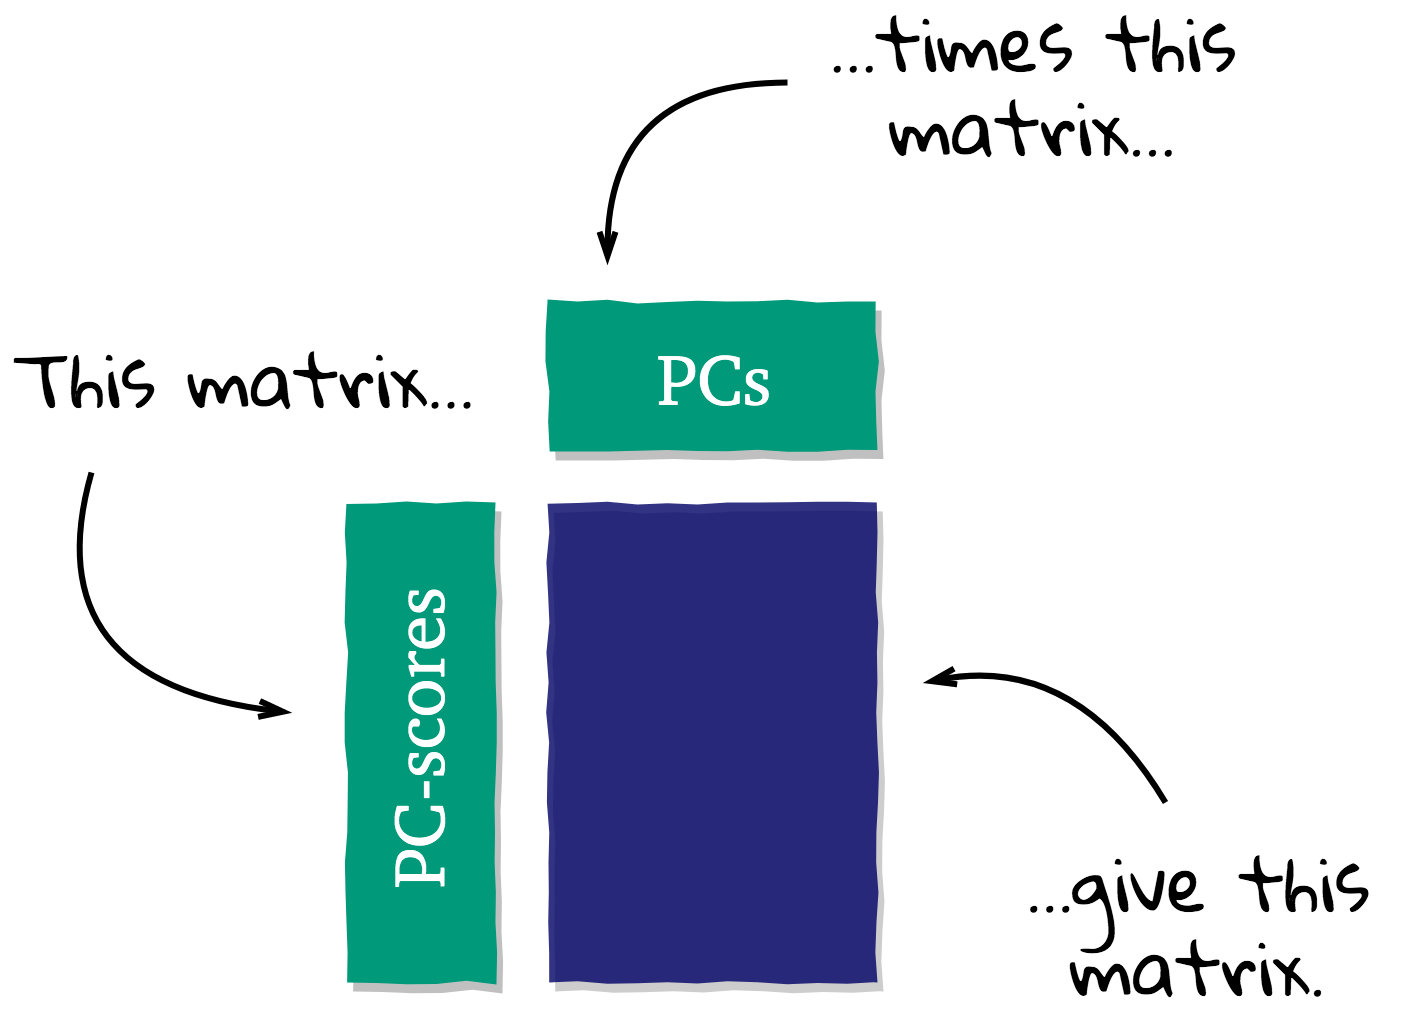
\includegraphics[width=7cm]{DWGs/matrix-multiplication-explanation.png}
%\caption{Matrix multiplication from eq.(\ref{eq:data-set-approximation}) shown graphically.}			
%\label{fig:matrix-multiplication-graphically}
%\end{figure}

It is worth noticing here that indeed the obtained matrices are necessarily rank-1, since they are formed as a linear combination of a single vector. This can be seen in two ways: either you may take the vector of PC-scores $(10 \times 1)$ and assume that it forms every column of the $(10 \times 6)$ matrix through multiplying it by the corresponding element from the PC vector. Or, you may assume that the PC is a vector that forms every row of the $(10 \times 6)$ matrix when multiplied by the corresponding element from the PC-scores vector. In either case, the full matrix $(10 \times 6)$ becomes a linear combination of a single vector - hence, it is rank-1.

\begin{figure}[H]
\begin{subfigure}[t]{.15\textwidth}
\centering
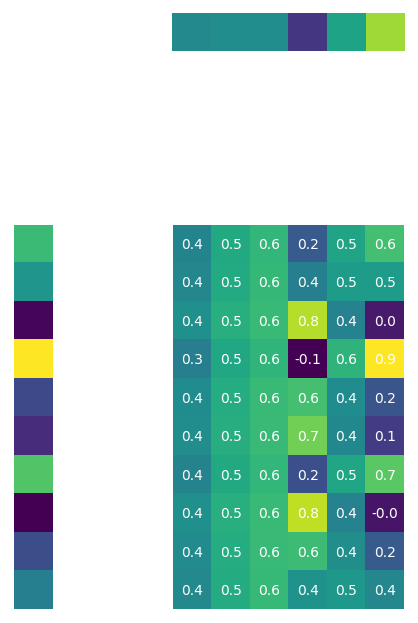
\includegraphics[scale=.2]{DWGs/random-matrix-reconstruction-PCs-1.png}
\caption{ }
\end{subfigure}
\begin{subfigure}[t]{.15\textwidth}
\centering
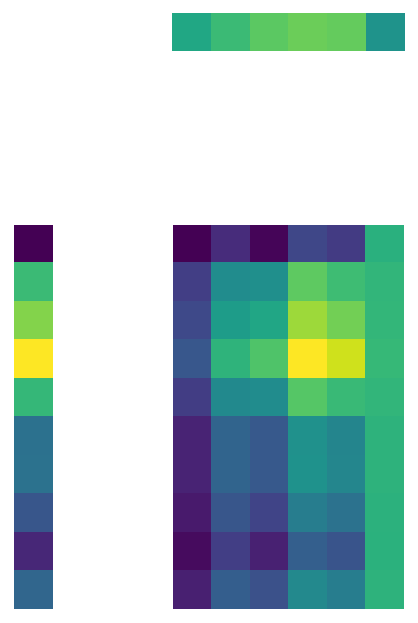
\includegraphics[scale=.2]{DWGs/semi-structured-matrix-reconstruction-PCs-1.png}
\caption{ }
\end{subfigure}
\begin{subfigure}[t]{.15\textwidth}
\centering
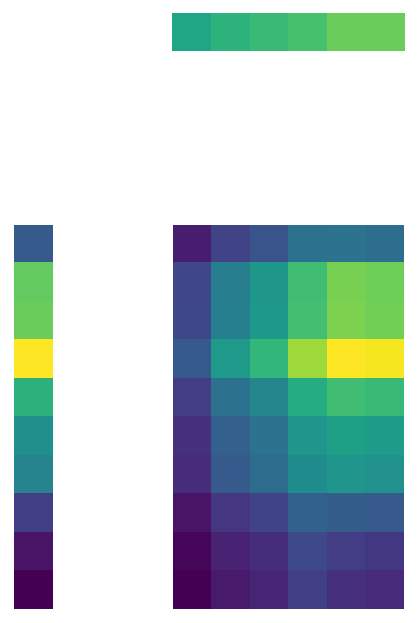
\includegraphics[scale=.2]{DWGs/structured-matrix-reconstruction-PCs-1.png}
\caption{ }
\end{subfigure}
\caption{Reconstruction with $1^{st}$ Principal Component of: (a) random matrix, (b) semi-structured matrix, (c) structured matrix.}
\label{fig:matrices-reconstruction-1}
\end{figure}

In Fig.\ref{fig:matrices-reconstruction-2} we present a rank-2 approximation, where we maintained two first PCs. Again, the matrices $(10 \times 2)$ represent the PC-scores and the vectors $(2 \times 6)$ represent the PCs.

In the semi-structured and structured matrix, the single matrix elements with highest numerical values (yellow) are already recovered in their actual positions. In the random matrix this is still not the case with rank 2-approximation.

Following the analogous reasoning as for Fig.\ref{fig:matrices-reconstruction-1} we may notice that the matrix reconstructed with two PCs is a rank-2 matrix.


\begin{figure}[H]
\begin{subfigure}[t]{.15\textwidth}
\centering
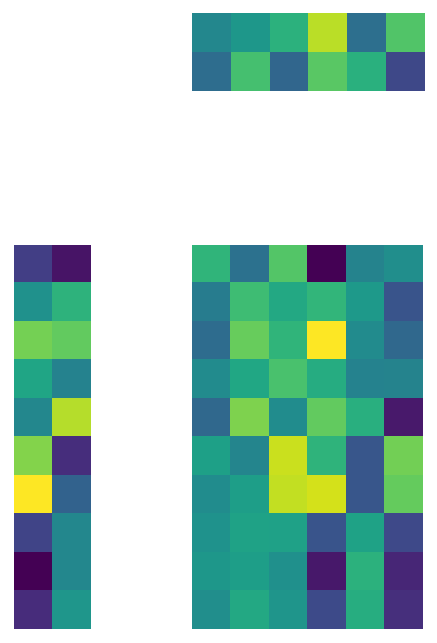
\includegraphics[scale=.2]{DWGs/random-matrix-reconstruction-PCs-2.png}
\caption{ }
\end{subfigure}
\begin{subfigure}[t]{.15\textwidth}
\centering
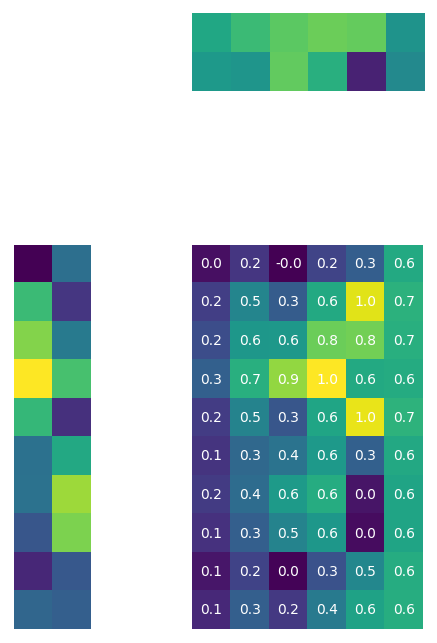
\includegraphics[scale=.2]{DWGs/semi-structured-matrix-reconstruction-PCs-2.png}
\caption{ }
\end{subfigure}
\begin{subfigure}[t]{.15\textwidth}
\centering
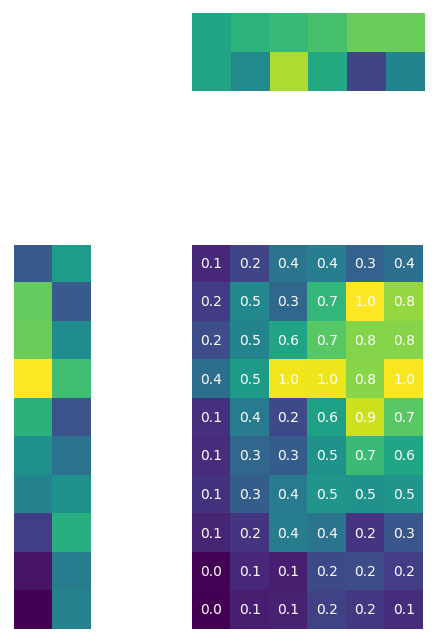
\includegraphics[scale=.2]{DWGs/structured-matrix-reconstruction-PCs-2.png}
\caption{ }
\end{subfigure}
\caption{Reconstruction with 2 Principal Components of: (a) random matrix, (b) semi-structured matrix, (c) structured matrix.}
\label{fig:matrices-reconstruction-2}
\end{figure}

The original data matrices are not completely retrieved until all 6 Principal Components and 6 PC-scores are taken into account. In Fig.\ref{fig:matrices-reconstruction-6} we obtain the final data matrices of rank-6.

The PC-scores are low-dimensional representations of the original data matrix and we return to the original dimensions by the transformation from eq.(\ref{eq:X-approximation}). In the case of taking all 6 PCs, the PC-scores $\bm{Z_q} = \bm{Z}$ and the eq.(\ref{eq:data-set-approximation}) becomes the eq.(\ref{eq:X-retrieval}), rather than the approximation from eq.(\ref{eq:X-approximation}).

\begin{figure}[H]
\begin{subfigure}[t]{.15\textwidth}
\centering
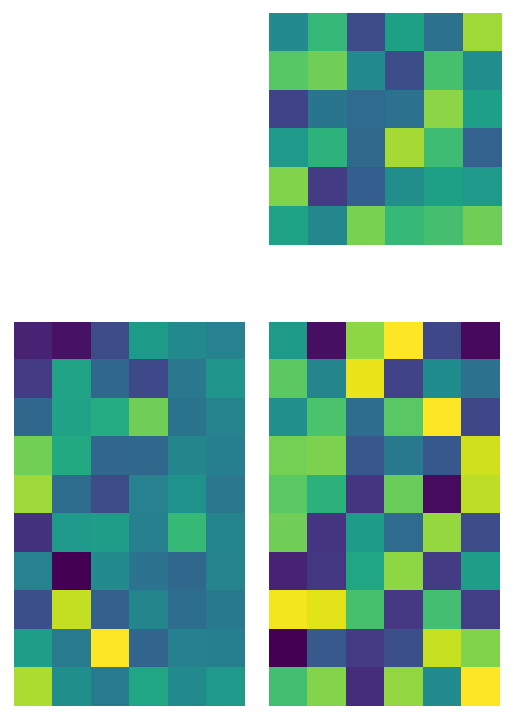
\includegraphics[scale=.2]{DWGs/random-matrix-reconstruction-PCs-6.png}
\caption{ }
\end{subfigure}
\begin{subfigure}[t]{.15\textwidth}
\centering
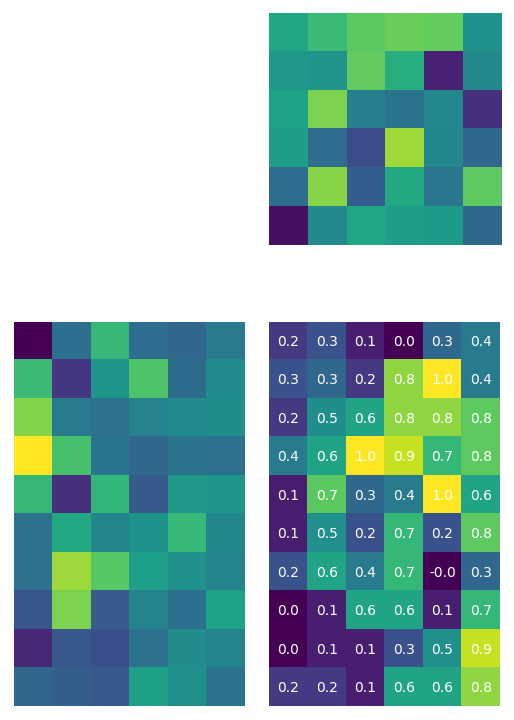
\includegraphics[scale=.2]{DWGs/semi-structured-matrix-reconstruction-PCs-6.png}
\caption{ }
\end{subfigure}
\begin{subfigure}[t]{.15\textwidth}
\centering
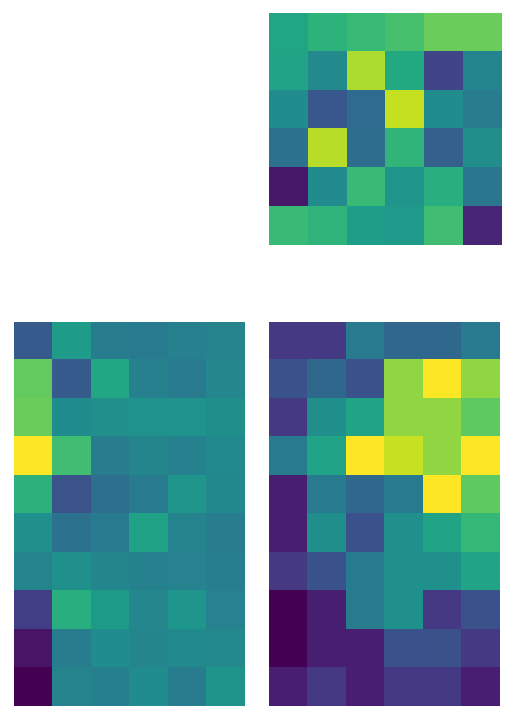
\includegraphics[scale=.2]{DWGs/structured-matrix-reconstruction-PCs-6.png}
\caption{ }
\end{subfigure}
\caption{Reconstruction with 6 Principal Components of: (a) random matrix, (b) semi-structured matrix, (c) structured matrix.}
\label{fig:matrices-reconstruction-6}
\end{figure}

Indeed, the multiplications from Fig.\ref{fig:matrices-reconstruction-6} show full PC-scores matrices transformed to the original 6 dimensions using the inverse (transposition) of the basis matrix made from PCs. The resulting matrix has to be the original data matrix.



\subsection{Local PCA}

PCA can also be applied on portions of the entire data set, in \textit{local clusters}. This can have certain advantages. Firstly, the reconstruction of the data set from low-rank approximations in the local clusters can allow for further reduction in dimensionality of a non-linear data set. This is due to the fact that clustering creates portions that are locally linear (or at least that are close to being linear). Secondly, the interpretation of Principal Components in local clusters can have more physical meaning, since they become better suited to represent that specific cluster.

Below is an example of the general idea of performing Local PCA. A data set composed of two distinct clouds of data can be first partitioned (for instance by techniques such as K-Means clustering) and then PCA is performed separately on both portions of the entire data set. What happens in practice is that the same PCA workflow is applied but on a subset of the data. Notice that the found PCs have different directions.

\begin{figure}[H]
\centering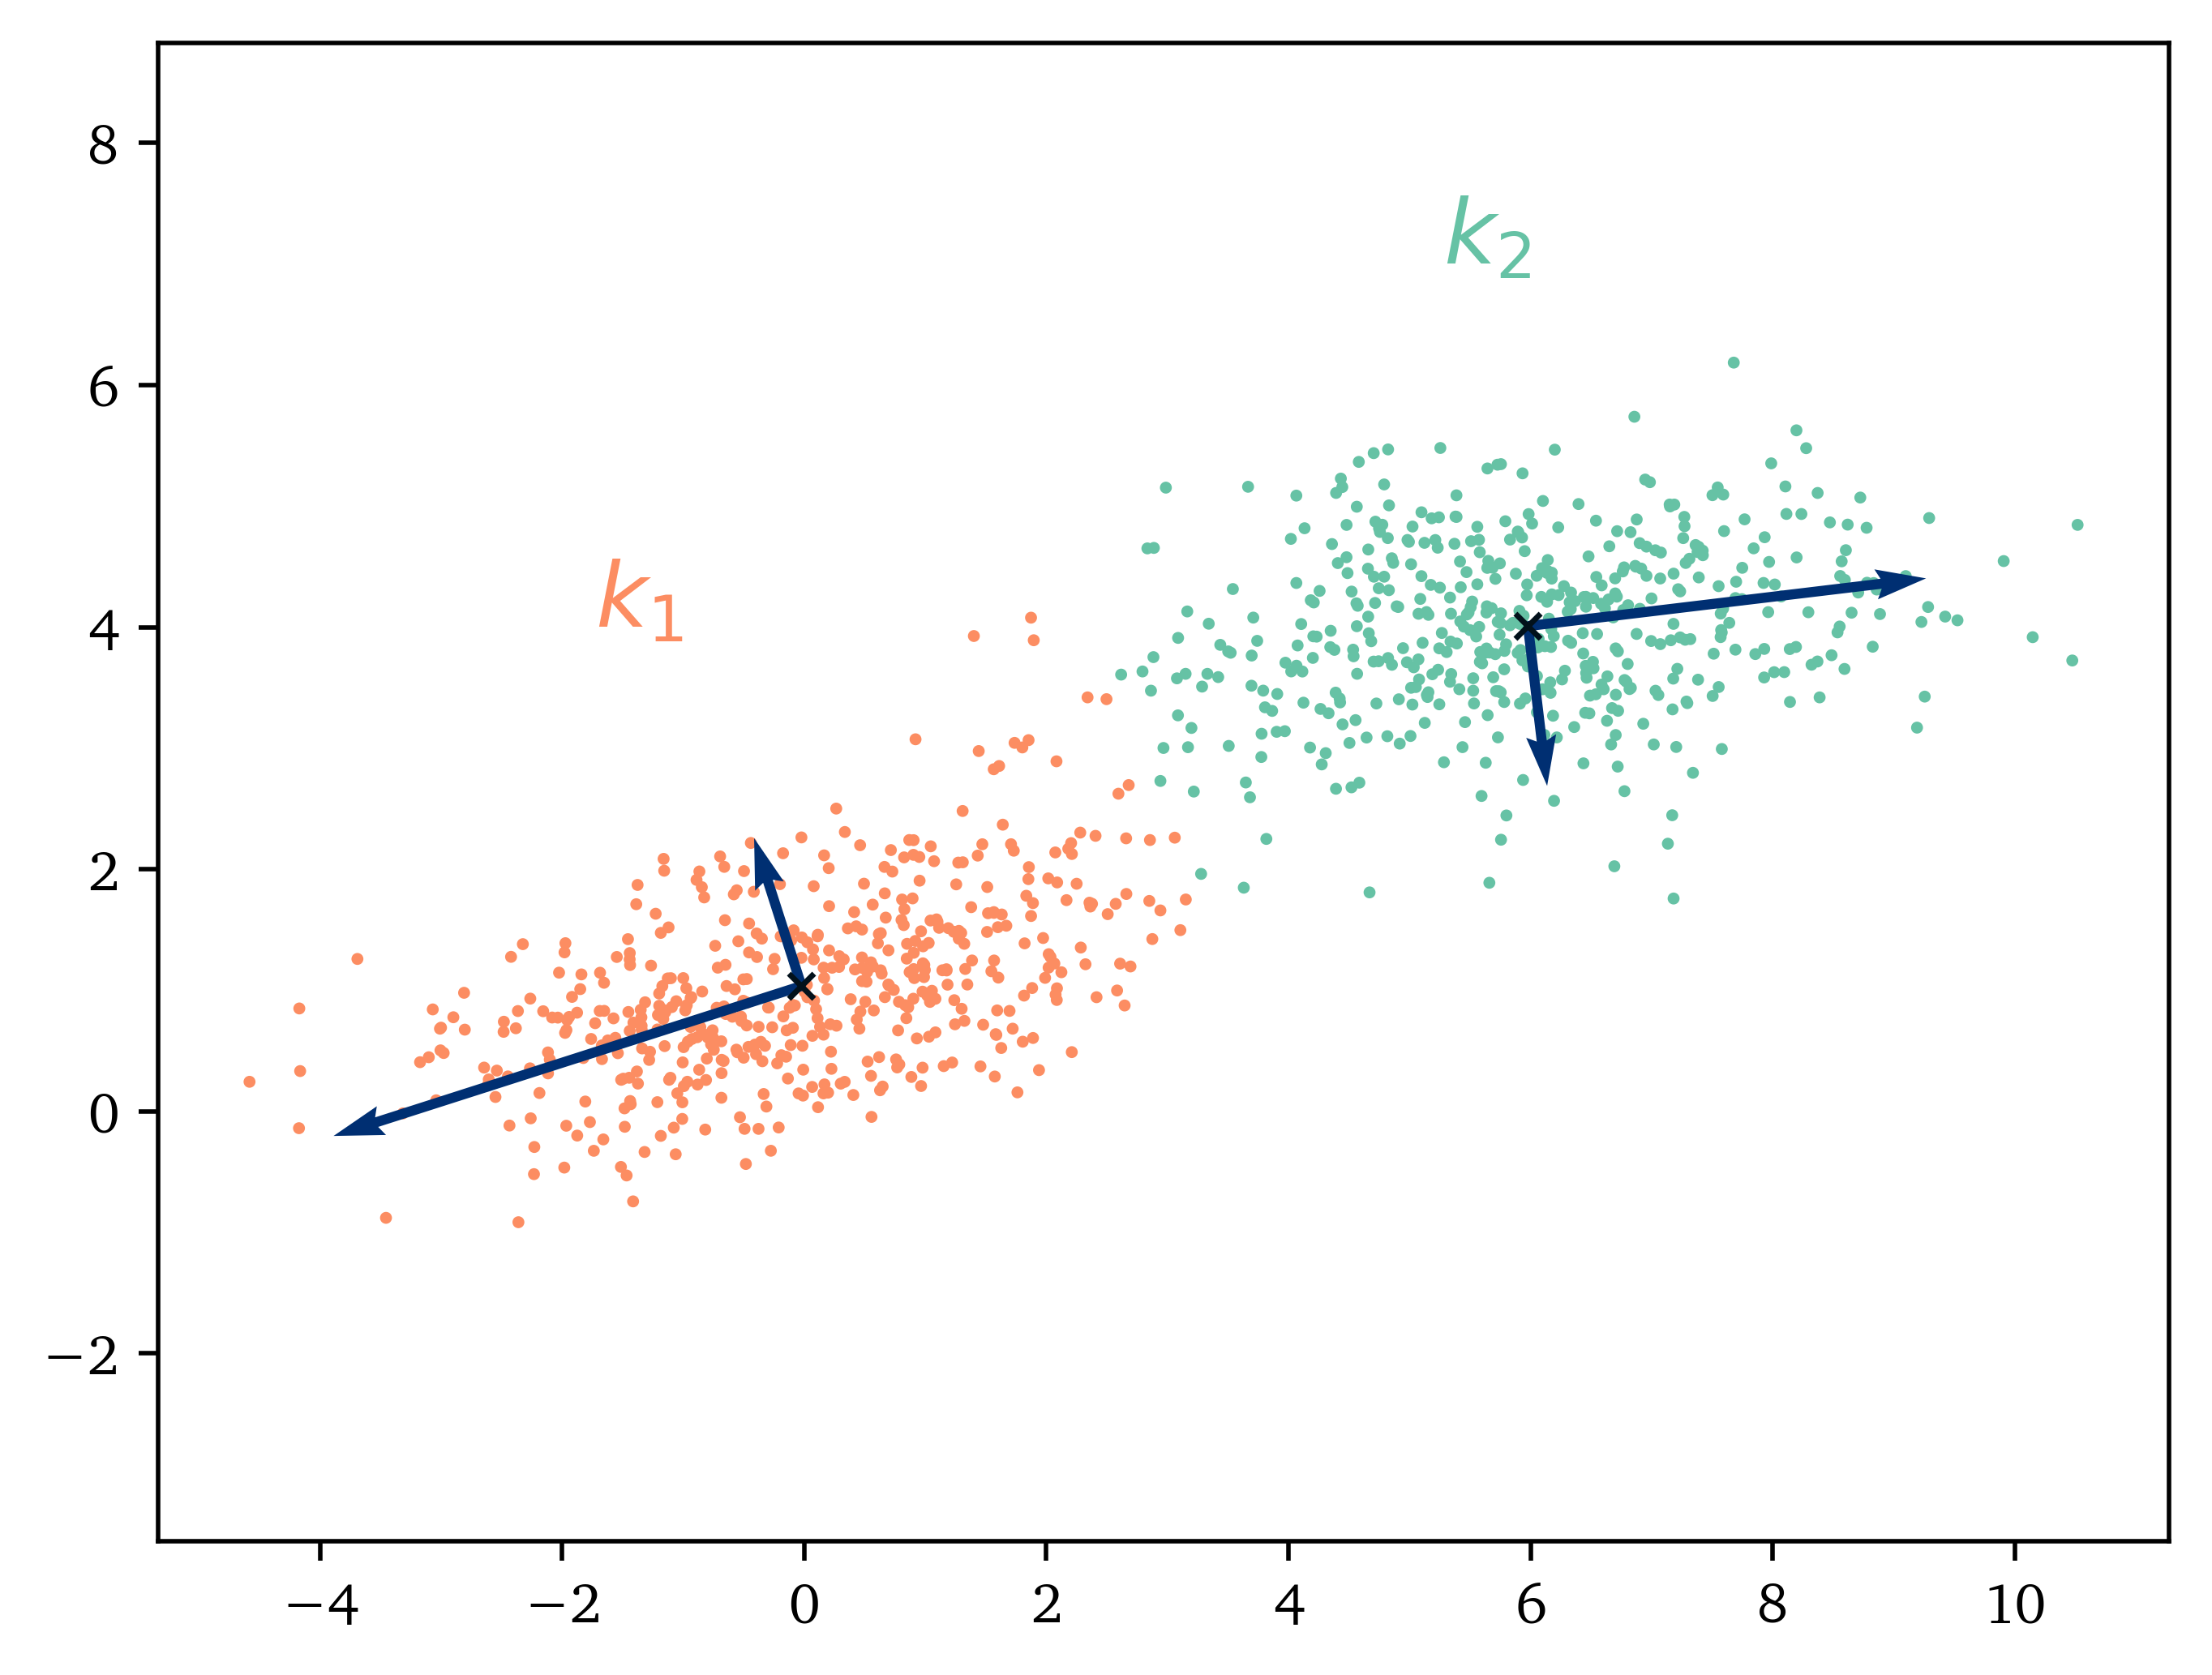
\includegraphics[width=8cm]{lpca-on-cloud-data.png}
\caption{Local PCA.}
\label{fig:local-pca}
\end{figure}

In the second example presented in the figure below we have a data set with a non-linear behaviour. Performing PCA on the entire data set will result in two PCs that will not represent very accurately the direction of variance of the most "bent" region at the top of the figure. You can observe that after dividing the data into three clusters the local PCs adjust to the direction of variance in each cluster.

\begin{figure}[H]
\centering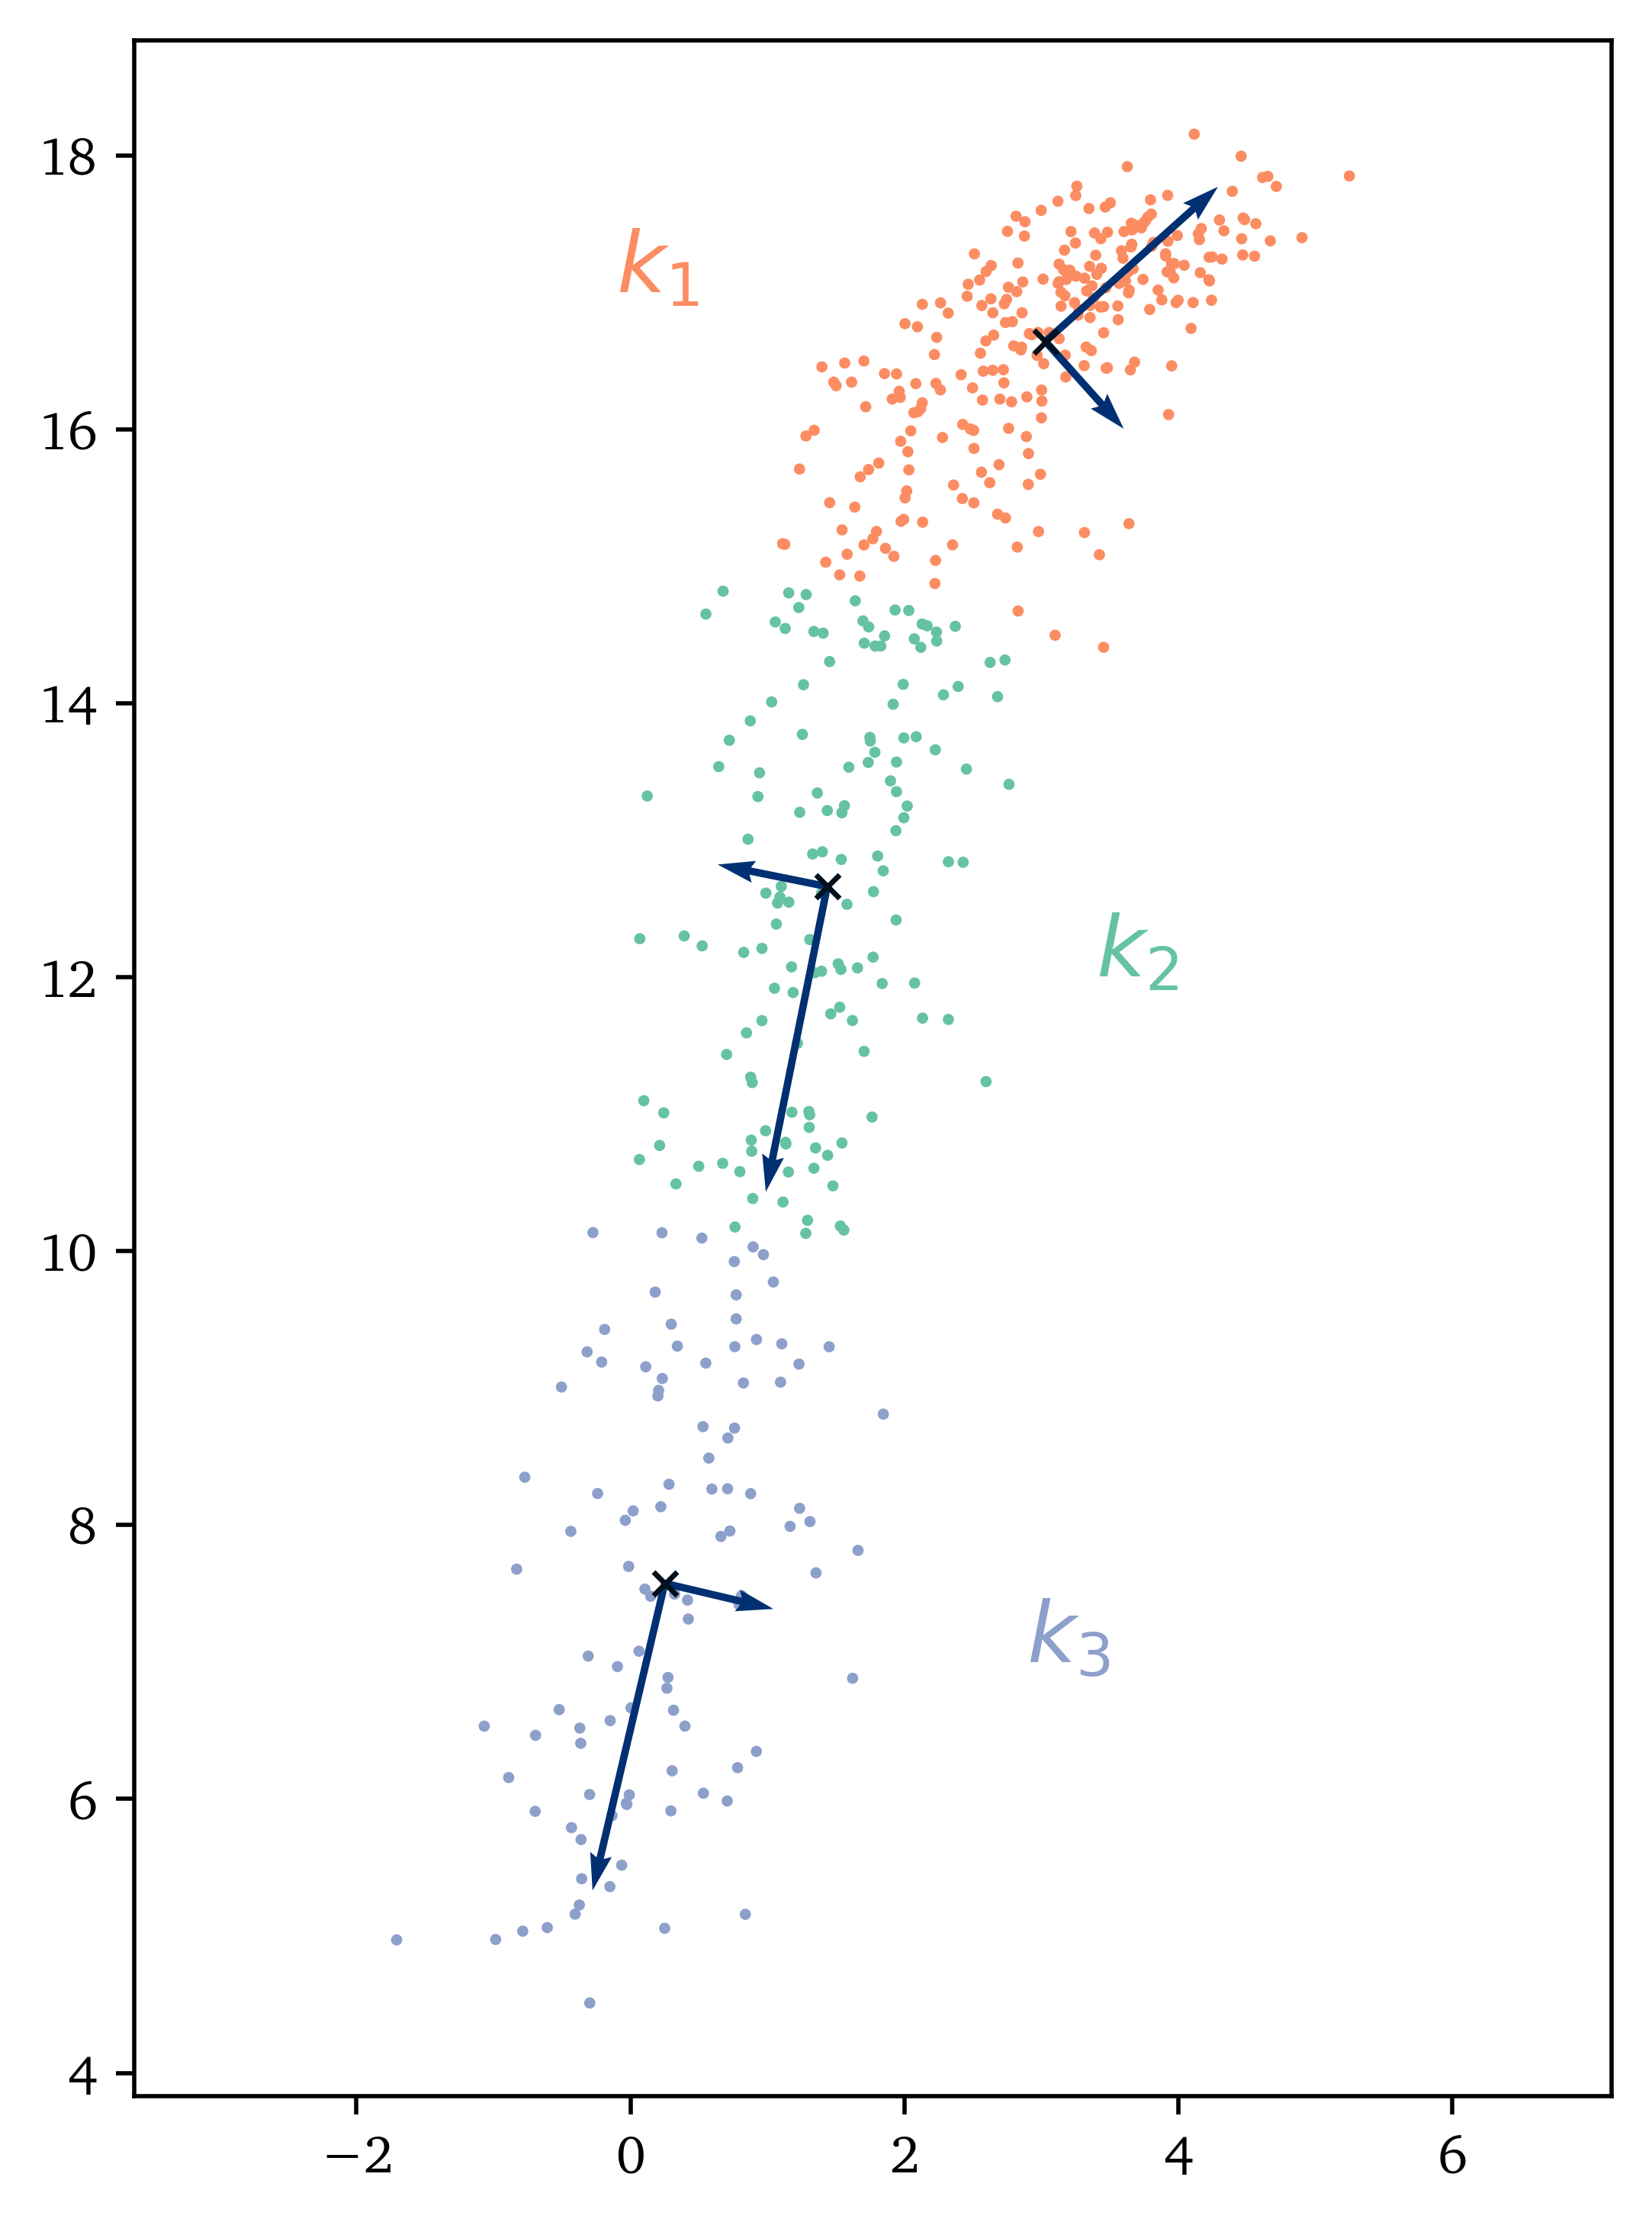
\includegraphics[width=6cm]{lpca-on-nonlinear-data.png}
\caption{Local PCA.}
\label{fig:local-pca}
\end{figure}

The reconstruction from the Local PCA is slightly more involved since now we have to account for contributions from each cluster separately.







\section{Questions to pause and ponder} \label{app:questions}

To give you a chance for further exposure to PCA,  here are a few questions for you to think about. Take a piece of paper and a pencil, or use your favourite programming language to explore these.

\begin{enumerate}
\item What happens if you did PCA on a rank-deficient matrix? Would it still find all the Principal Components? And if yes, what's the meaning of that...? What would the eigenvalues look like?
\item What happens if the columns of the original data matrix $\bm{X}$ are \textit{very close} to being linearly dependent? What I mean by that is, let's assume that matrix $\bm{X}$ is still of full-rank, but each column is approximately a linear combination of some other column.
\item What happens if you do PCA on a \textit{ring} data set like the one in Fig.\ref{fig:ring-data-set}?
\begin{figure}[H]
\centering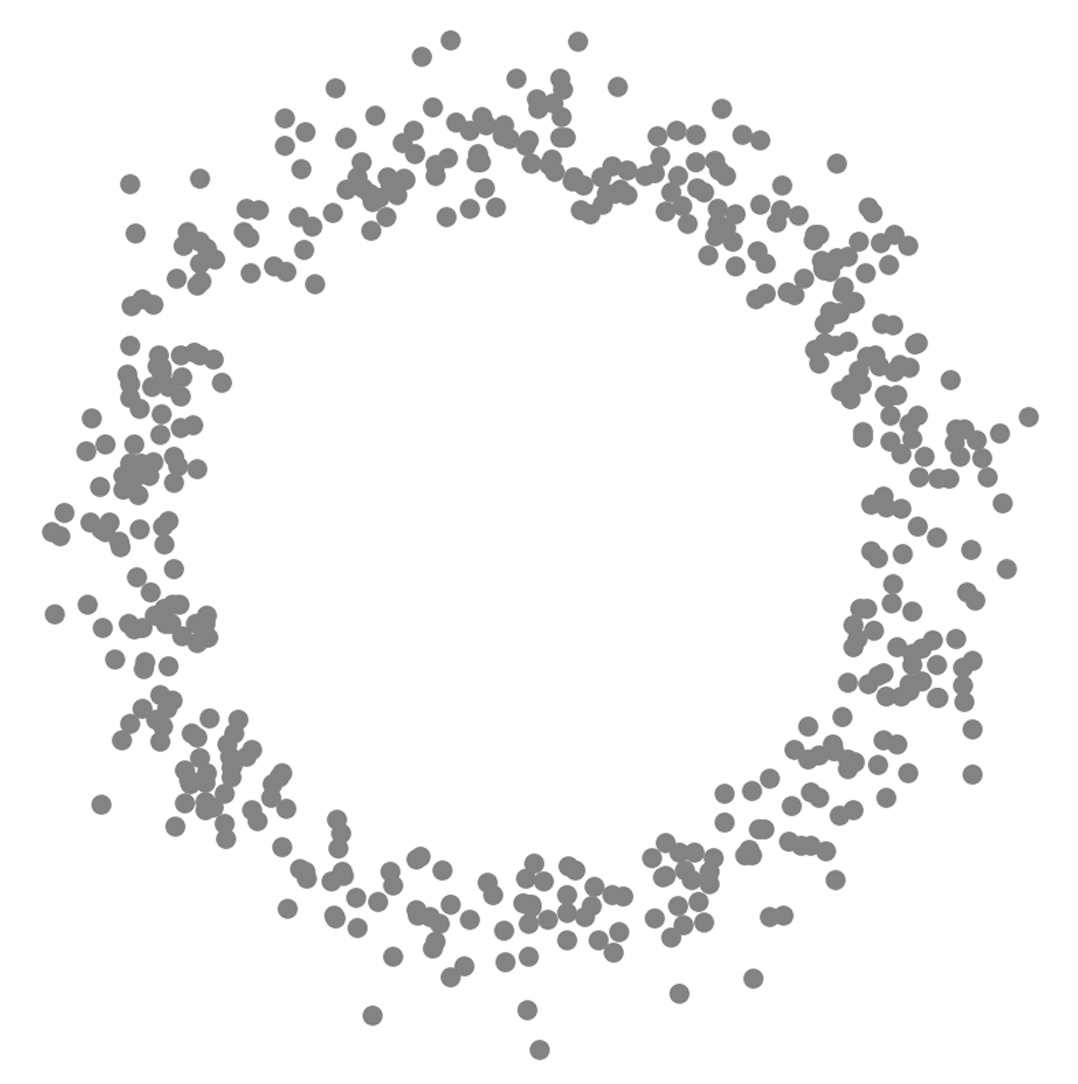
\includegraphics[width=4cm]{ring-data-set.png}
\caption{Ring data set.}
\label{fig:ring-data-set}
\end{figure}
\item What would the original data set $\bm{X}$ have to be so that the PCs found are the standard basis vectors?
\end{enumerate}

%\subsection{The intuition behind $\frac{1}{n - 1}$.}


%\subsection{Statistical independence}


%The Principal Components are linearly independent (since they are orthogonal) but it does not mean that they are statistically independent. This is one of the limitations of PCA.

\thebibliography{}

\bibitem{Abdi_Williams} Herve Abdi, Lynne J. Williams, \textit{Principal component analysis}, 2010
\bibitem{3Blue1Brown} 3Blue1Brown, \textit{Essence of linear algebra}
\bibitem{Matlab-pca} https://nl.mathworks.com/help/stats/pca.html
\bibitem{Python-pca} https://scikit-learn.org/stable/modules/generated/
sklearn.decomposition.PCA.html
\bibitem{eckart-young} C. Eckart, G. Young, \textit{The approximation of one matrix by another of lower rank}, 1936, Psychometrika, 1 (3) 211-218
\bibitem{Jolliffe} Ian T. Jolliffe, \textit{Principal Component Analysis}, Second Edition, 1986
\bibitem{Strang} Gilbert Strang, \textit{Introduction to Linear Algebra}, Fifth Edition, 2016
\bibitem{Shlens} Jonathon Shlens, \textit{A Tutorial on Principal Component Analysis}, 2016, https://arxiv.org/abs/1404.1100
\bibitem{cov-dot} http://people.sju.edu/~pklingsb/dot.cov.pdf
\bibitem{Jackson} J. Edward Jackson, \textit{A User's Guide To Principal Components}, 1991
\bibitem{Smith} Lindsay I. Smith, \textit{A tutorial on Principal Component Analysis}, 2002

\bibitem{Shalizi} Cosma Shalizi, Course on statistics: \textit{The Truth about Principal Components and Factor Analysis}, 2009 https://www.stat.cmu.edu/~cshalizi/350/



\end{document}
